% Copyright 2004 by Till Tantau <tantau@users.sourceforge.net>.
%
% In principle, this file can be redistributed and/or modified under
% the terms of the GNU Public License, version 2.
%
% However, this file is supposed to be a template to be modified
% for your own needs. For this reason, if you use this file as a
% template and not specifically distribute it as part of a another
% package/program, I grant the extra permission to freely copy and
% modify this file as you see fit and even to delete this copyright
% notice.
\documentclass[notes]{beamer}
% There are many different themes available for Beamer. A comprehensive
% list with examples is given here:
% http://deic.uab.es/~iblanes/beamer_gallery/index_by_theme.html
% You can uncomment the themes below if you would like to use a different

%\usetheme{AnnArbor}
%\usetheme{Antibes}
%\usetheme{Bergen}
%\usetheme{Berkeley}
%\usetheme{Berlin}
%\usetheme{Boadilla}
%\usetheme{boxes}
%\usetheme{CambridgeUS}
%\usetheme{Copenhagen}
%\usetheme{Darmstadt}
%\usetheme{default}
%\usetheme{Frankfurt}
%\usetheme{Goettingen}
%\usetheme{Hannover}
%\usetheme{Ilmenau}
%\usetheme{JuanLesPins}
%\usetheme{Luebeck}
%\usetheme{Madrid}
%\usetheme{Malmoe}
%\usetheme{Marburg}
%\usetheme{Montpellier}
%\usetheme{PaloAlto}
%\usetheme{Pittsburgh}
%\usetheme{Rochester}
%\usetheme{Singapore}
%\usetheme{Szeged}
%\usetheme{Warsaw}
%\usetheme[]{metropolis}

\title{A Lagrangian geography of the deep\\Gulf of Mexico}

% A subtitle is optional and this may be deleted
%\subtitle{Optional Subtitle}

\author{Philippe Miron\inst{1},  Francisco J. Beron-Vera\inst{1}, Mar\'ia J. Olascoaga\inst{1}, J.\ Sheinbaum\inst{2}, P.\ P\'erez-Brunius\inst{2} and Gary Froyland\inst{3}}
\institute
{
  \inst{1}%
  RSMAS University of Miami, Miami, USA
  \and
  \inst{2}
  CICESE, Ensenada, Mexico
  \and
  \inst{3}%
  University of New South Wales, Sydney, Australia
  }
% - Use the \inst command only if there are several affiliations.
% - Keep it simple, no one is interested in your street address.

\date{Ocean Sciences Meeting on Wednesday, February 14 2018}
% - Either use conference name or its abbreviation.
% - Not really informative to the audience, more for people (including
%   yourself) who are reading the slides online

\subject{Applied oceanography}
% This is only inserted into the PDF information catalog. Can be left
% out. 

% Beamer settings
\setbeamertemplate{navigation symbols}{} %remove nav symbols
\setbeamertemplate{bibliography item}{}
\setbeamertemplate{footline}[frame number]

% If you have a file called "university-logo-filename.xxx"
% is a graphic format that can be processed by latex or pdflatex,
% resp., then you can add a logo as follows:
%\pgfdeclareimage[height=1.5cm]{logo}{figures/GoMRi.png}
%\logo{\pgfuseimage{logo}}

% Delete this, if you do not want the table of contents to pop up at
% the beginning of each subsection:
%\AtBeginSubsection[]
%{
%  \begin{frame}<beamer>{Outline}
%  \tableofcontents[currentsection,currentsubsection]
%  \end{frame}
%}

% graphic
\graphicspath{{"2018. deep floats (agu)/figures/"}}
%\graphicspath{{"figures/"}}

% titlepage logo
\titlegraphic{
\begin{tikzpicture}[overlay, remember picture]
%\node[at=(current page.south west), anchor=south west] {%
% 
\includegraphics[height=.10\textwidth]{carthe.png} 
%};
\node[at=(current page.south west), anchor=south west] {%
 
\includegraphics[height=.18\textwidth]{cigom.jpg} 
};
\node[at=(current page.south east), anchor=south east] {
 
\includegraphics[height=.14\textwidth]{um-rsmas.png}
};
\end{tikzpicture}
}

% bibliography
\usepackage[style=authoryear, natbib=true]{biblatex}
\addbibresource{oce.bib}
% remove annoying biblatex bug/warning
\usepackage{silence}
\WarningFilter{biblatex}{Patching footnotes failed}

% some definitions
\usepackage[utf8]{inputenc}
\usepackage[english]{babel}
\usepackage{amssymb}
\usepackage{amsfonts}
\usepackage{amsmath}
\usepackage{bbold}
\usepackage{ragged2e} % justify text in all frame
\apptocmd{\frame}{}{\justifying}{}
\usepackage{etoolbox}
\usepackage{tikz}
\usepackage{subfig}
\usepackage{multicol}
\usepackage{siunitx}
\usepackage{csquotes}
\usepackage{hyperref}
\usepackage{tikz,pgfplots}
\pgfplotsset{compat=1.12}

% Definitions.
\DeclareMathOperator{\area}{area}%
\DeclareMathOperator{\Id}{Id}%
\newcommand{\PF}{\mathcal{P}}
\newcommand{\ia}{\textit{a}}
\newcommand{\ib}{\textit{b}}
\newcommand{\ic}{\textit{c}}
\newcommand{\id}{\textit{d}}
\newcommand{\ie}{\textit{e}}
\newcommand{\gom}{GoM}
\let\vaccent=\v 
\renewcommand{\v}[1]{\ensuremath{\mathbf{#1}}} 
\newcommand{\minus}{\scalebox{0.5}[1.0]{$-$}}
\newcommand{\dif}{\ensuremath{\text{d}}}

% Let's get started
\begin{document}

\frame[plain,noframenumbering]{
\titlepage
}

\iffalse
\begin{frame}{Outline}
  \tableofcontents
  % You might wish to add the option [pausesections]
\end{frame}
\fi

\section{Introduction}

\frame{\frametitle{Introduction}
Over the last twenty five years, many satellite-tracked surface drifters sampled the surface of the Gulf of Mexico (\gom). From a database of 3300 drifters, we presented a Lagrangian geography of the \gom.

\begin{figure}
    \centering
    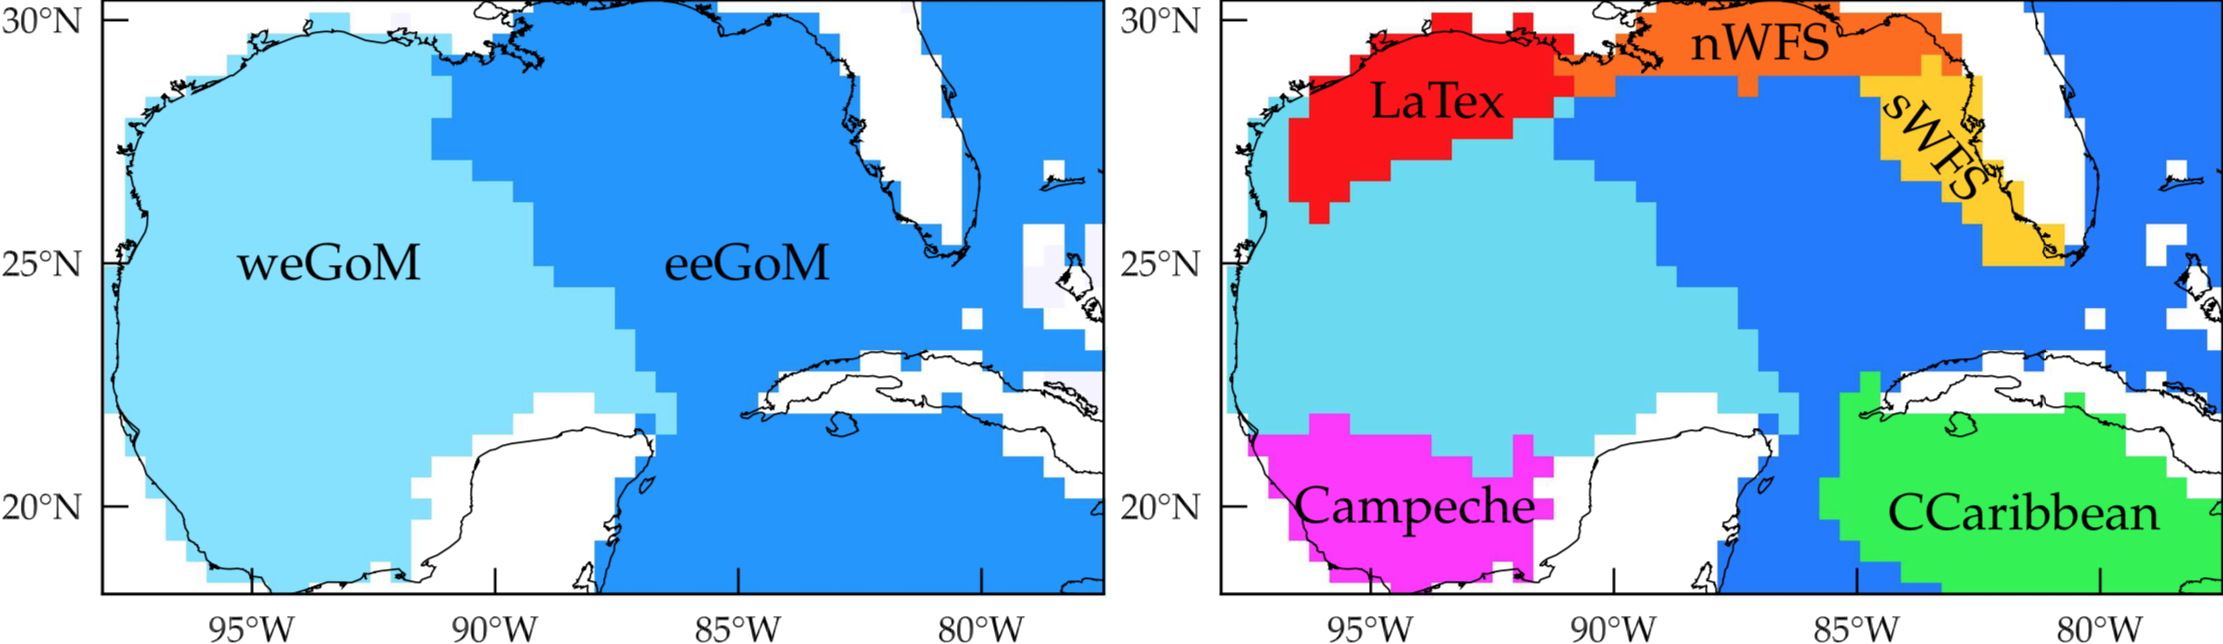
\includegraphics[width=\textwidth]{geosurf.png}
    \caption{Published in \cite{miron2017lagrangian}}
    \label{fig:geosurf}
\end{figure}
}

\frame{\frametitle{Introduction}
In contrast, very few studies were aimed at the characterization of the deep water global circulation. 
\newline\newline
RAFOS experiment sponsored by the Bureau of Ocean Energy Management (July 2011 - May 2015):
\begin{itemize}
\item 4-year-long program (floats $\sim 2$-y mission)
\item 121 floats at 1500\,m
\item 6 profiling floats with RAFOS technology at 1500\,m
\item 31 floats at 2500\,m

\end{itemize}

\textit{Publicly available data sets compiled by WOCE Subsurface Float Data Assembly Center (WFDAC).}\footnote{\url{http://www.aoml.noaa.gov/phod/float_traj/data.php}}
}

\section{Objectives}

\frame{\frametitle{Objectives}
Using floats data (trajectories) in the abyssal Gulf of Mexico (\gom):
\begin{itemize}
    \item subdivide the deep \gom\ into regions with similar dynamics;
    \item identify almost invariant region and their respective timescale;
    \item predict transport of \textit{passive tracers}.
\end{itemize}
}

\frame{\frametitle{Theory: transfer operator $\mathcal{P}$}
We want to predict at a time $T$ the dispersion of a an initial density $\rho(x,0) = f(x)$.
\newline\newline
This is given by the push forward of f(x),
\begin{equation}
    \rho(x,T) = \int_X f(y) k(x,y) \dif y = \mathcal{P}\,f(x)
\end{equation}
under the action of an advection-diffusion process that can be described via a bounded stochastic kernel $k$.

}

\note{Note that it is independant of initial T}

\frame{\frametitle{Theory: transfer operator $\mathcal{P}$}

\textcolor{red}{clean this}
A discretization of the transfer operator can be attained using a Galerkin approximation referred to as Ulam's method\cite{ulam1960}. This involves partitioning the domain $X$ into a grid of $N$ connected boxes $\{B_1,\dotsc,B_N\}$ and projecting functions in $L^1(X)$ onto a finite-dimensional space approximating $L^1(X)$ and spanned by indicator functions on the grid.

We assume from now on that the grid is regular, i.e., $\area(B_i)
= \area(B_j)$ for all $i\neq j$.
}





\frame{\frametitle{Theory: how to construct the transition matrix}  

By considering a sufficiently large number of initial conditions we can estimate the entries:
\begin{equation}
   P_{ij} = \frac{\# x \text{ in }B_i\text{ at any time } t \text{ and in }B_j \text{ at  } t+T}{\#x\text{ in }B_i \text{ at any time }t}.
  \label{eq:Pnum}
\end{equation}

The entries of $P$ can be viewed as transitional probabilities of moving from $B_i$ to $B_j$. It defines a \textbf{Markov Chain} (with bins $\equiv$ states) of the dynamics.
}

\frame{\frametitle{Application of the transition matrix}
One can push forward discrete representations of $f(x)$:
\begin{equation}
    \mathbf f = (f_1,\cdots,f_N),
\end{equation}
by right-multiplication by $P$:
\begin{align}
    f^{(1)} &= f\,P \nonumber\\
    f^{(2)} &= f^{(1)}\,P = f\,P^2 \nonumber\\
    f^{(k)} &= f\,P^k
\end{align}

Similarly, we push backward an initial distribution using $P^\top$.
}

\frame{\frametitle{Eigenvectors analysis}

It is also of interest to identify when a distribution $\mathbf f$ is almost invariant:
\begin{equation}
    \mathbf f \approx \mathbf f\,P
\end{equation}

This is available from the \emph{eigenspectrum} inspection of $P$ \citep{Froyland-etal-12}.
\newline\newline
If in the matrix $P$:
\begin{itemize}
    \item all states \emph{communicate};
    \item no state occurs \emph{periodically}.
\end{itemize}
$P$ has a limiting distribution $\mathbf{p} = \mathbf{p} P$.
\newline\newline
Note: $\mathbf{p}$ is a left eigenvector of $P$ with eigenvalue $\lambda = 1$ ($\mathbf{p} \lambda = \mathbf{p} P$). Because of row-stochasticity of $P$, the corresponding right eigenvector is $\mathbb{1}$, i.e., $P\mathbb{1} = \mathbb{1}$.
}

\frame{\frametitle{Attractors and basin of attractions}
Any distribution $f_\mathbb{1}$ supported on the right eigenvector $\mathbb{1}$ will converge to $\mathbf{p}$ as the number of applications of $P$ tends to infinity, i.e., $\smash{\lim_{n \to \infty} f_\mathbb{1}P^n = \mathbf{p}}$.
\newline\newline
For $\lambda = 1$:
\begin{itemize}
    \item right eigenvector of $P$ is the basin of attraction
    \item left eigenvector of $P$ is the attractor
\end{itemize}

This motivates the idea that regions where trajectories converge and their basins of attraction are encoded in the eigenvectors of the transition matrix $P$ with eigenvalues ($\lambda \approx 1$) \citep{froyland2014well}.
}

\frame{\frametitle{Data}
Trajectories of the RAFOS cover the area under 1500\,m of the Gulf of Mexico.
\begin{figure}
  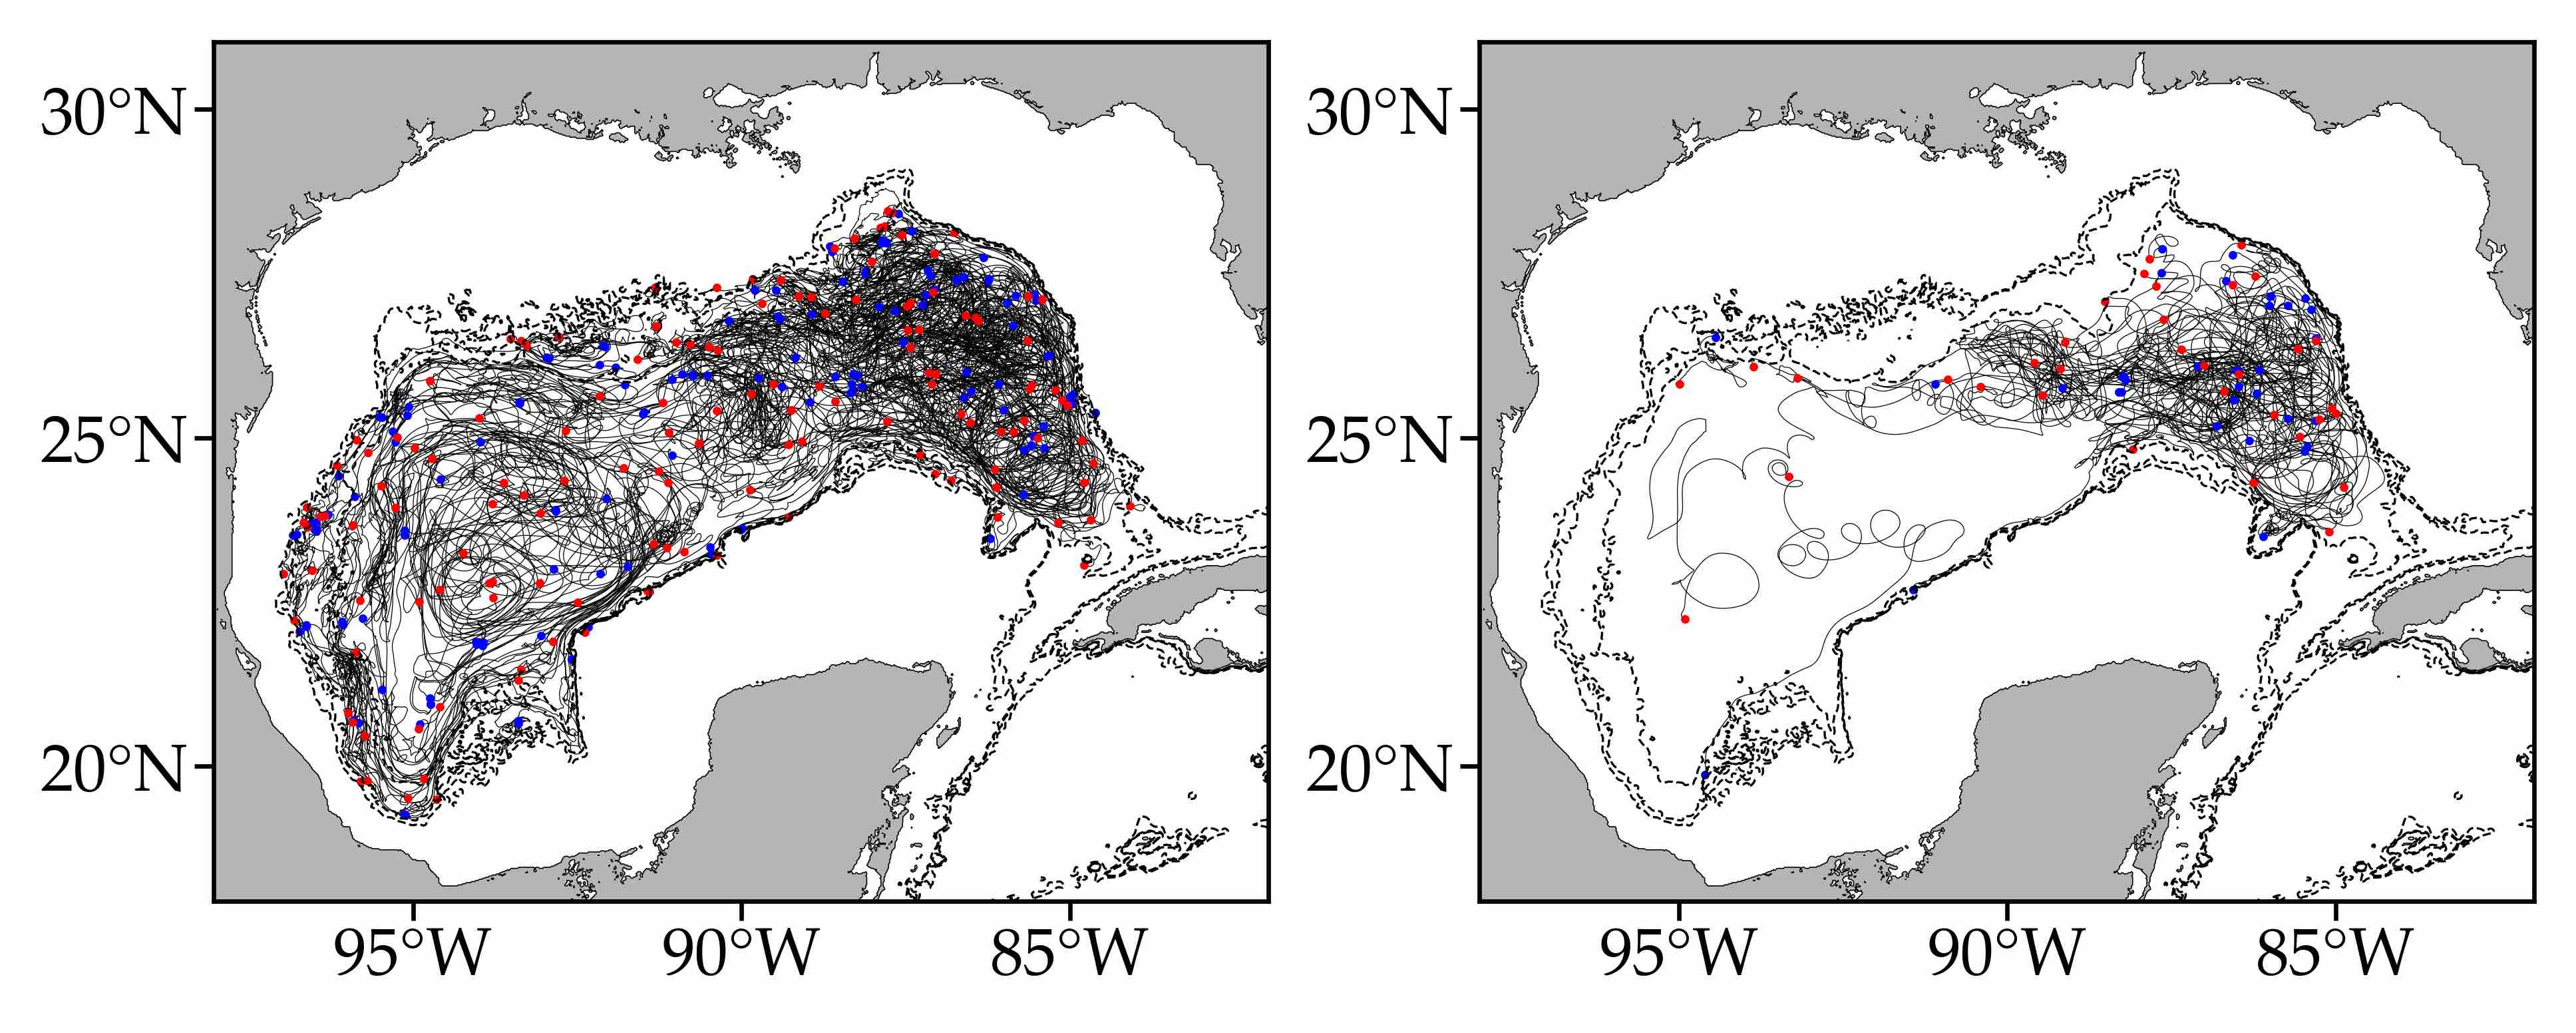
\includegraphics[width=\textwidth]{geogomdeep-fig01.jpg}
\end{figure}
}

\section{Results}
\frame{\frametitle{Eigenvectors}

\only<1>{
Eigenvectors associated with $\lambda_1=1$ and $\lambda_2=0.9953$.
\begin{figure}
  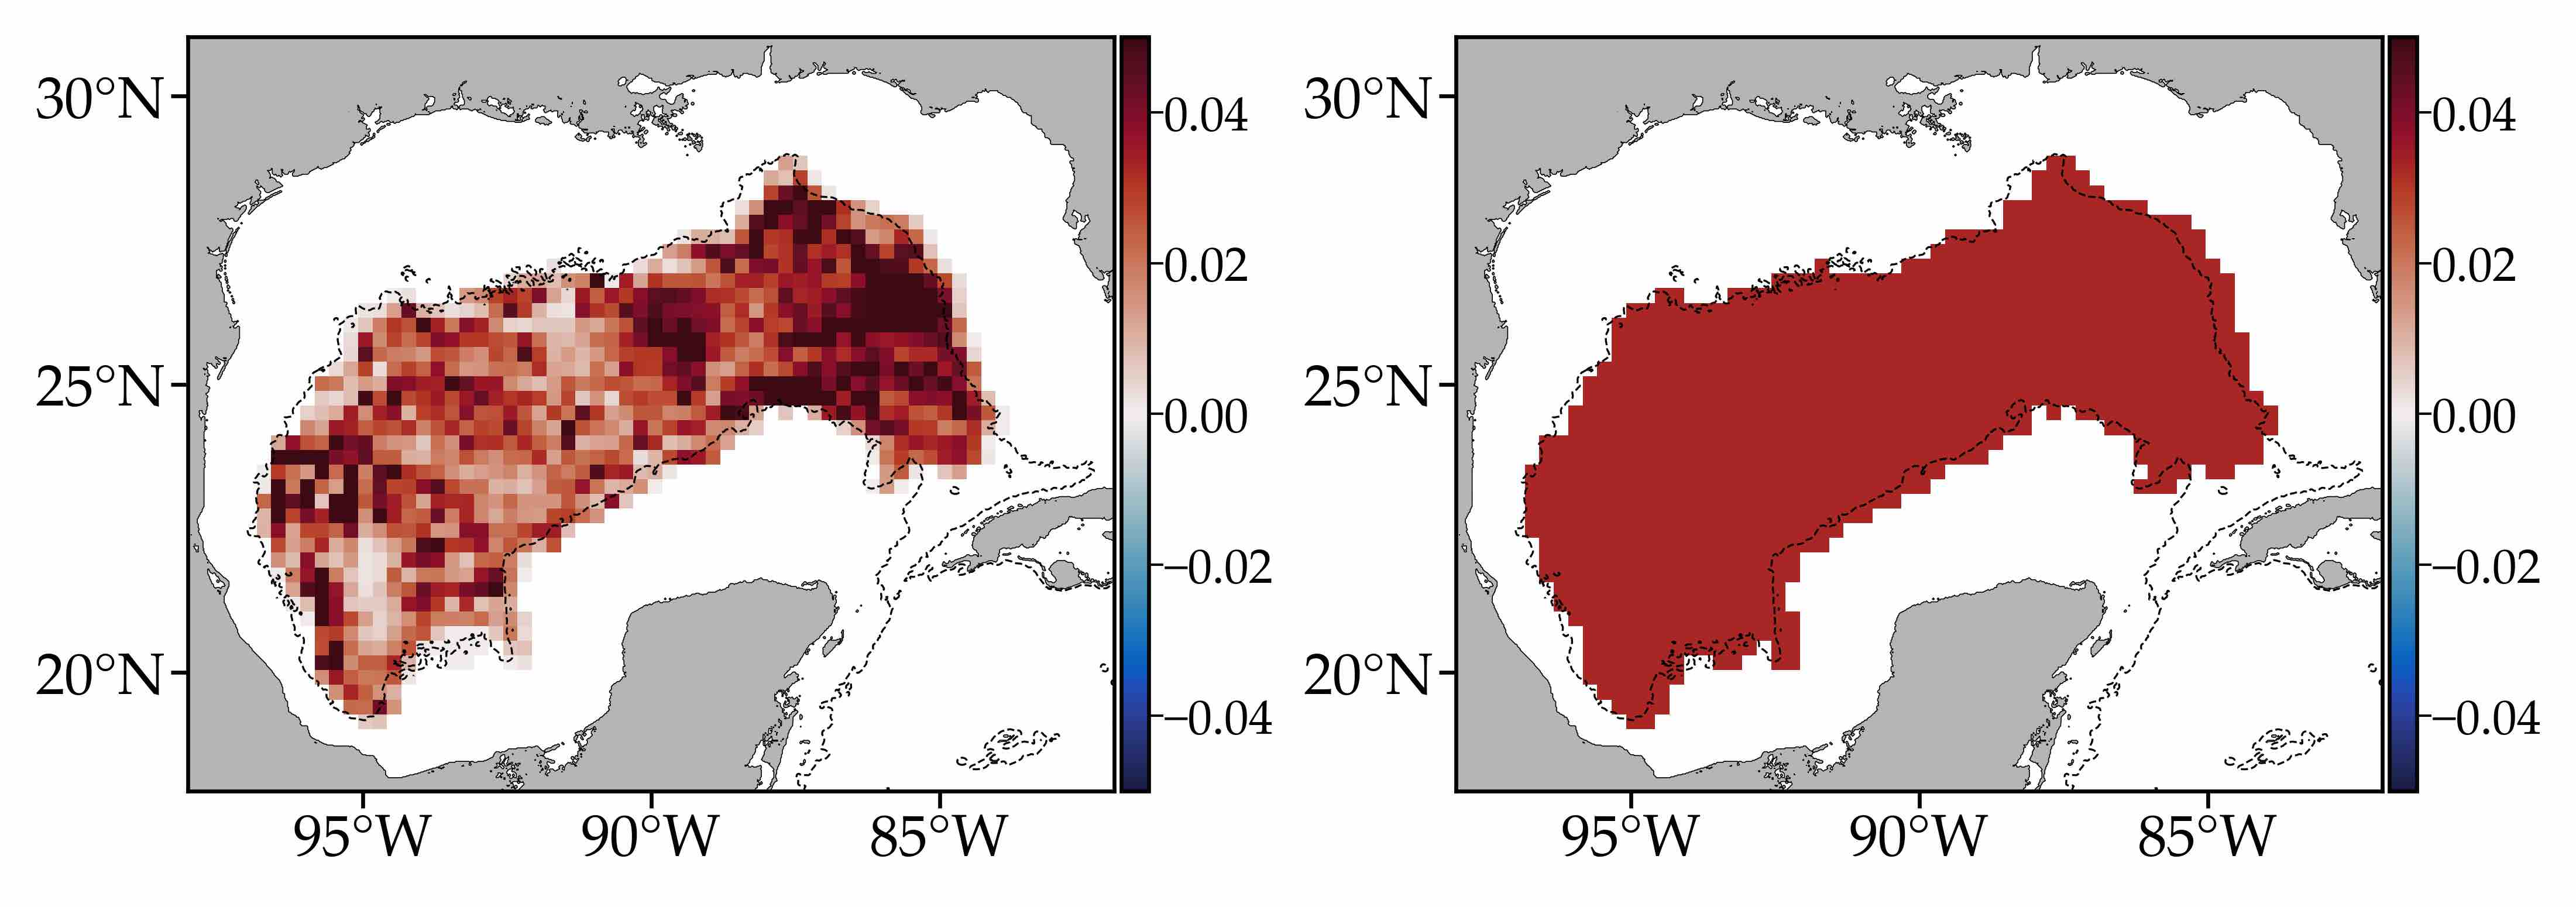
\includegraphics[width=\textwidth]{geogomdeep-fig07.jpg}
\end{figure}
\begin{figure}
  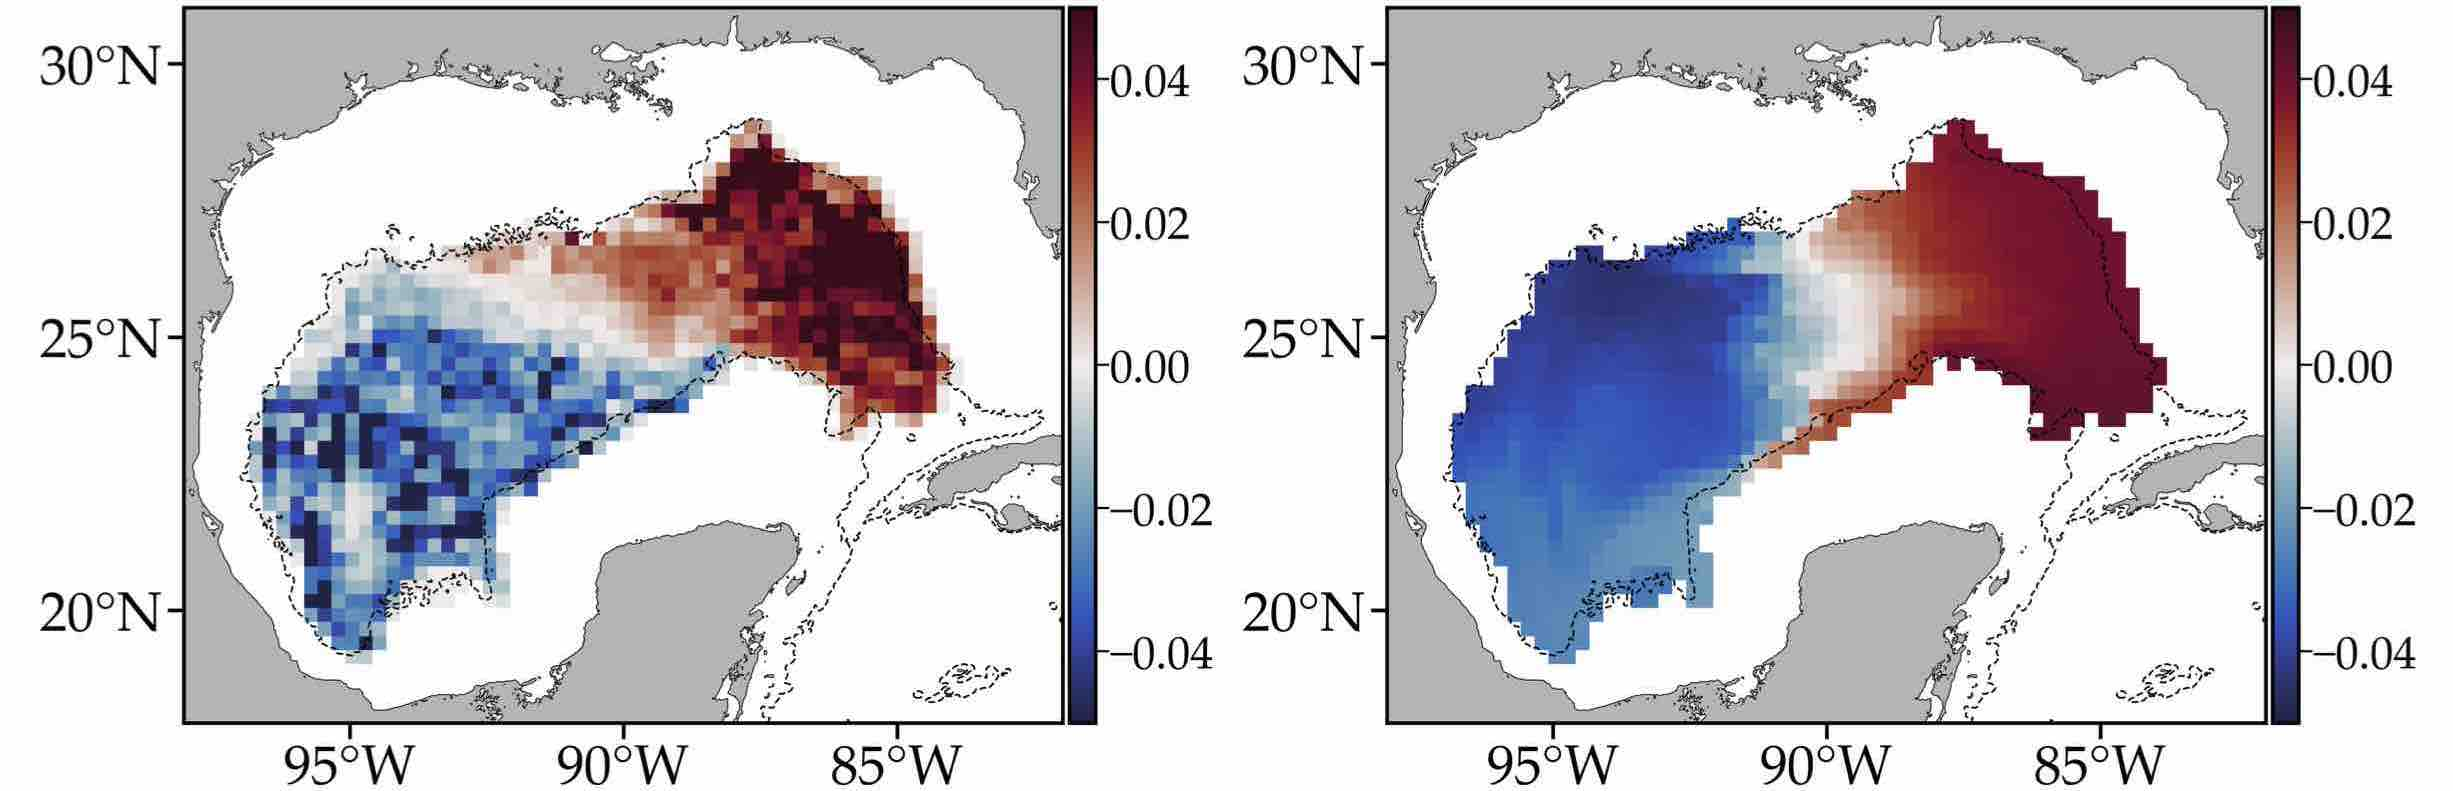
\includegraphics[width=\textwidth]{geogomdeep-fig08a.jpg}
\end{figure}
}

\only<2>{
Eigenvectors associated with $\lambda_3=0.9832$ and $\lambda_5=0.9712$.
\begin{figure}
  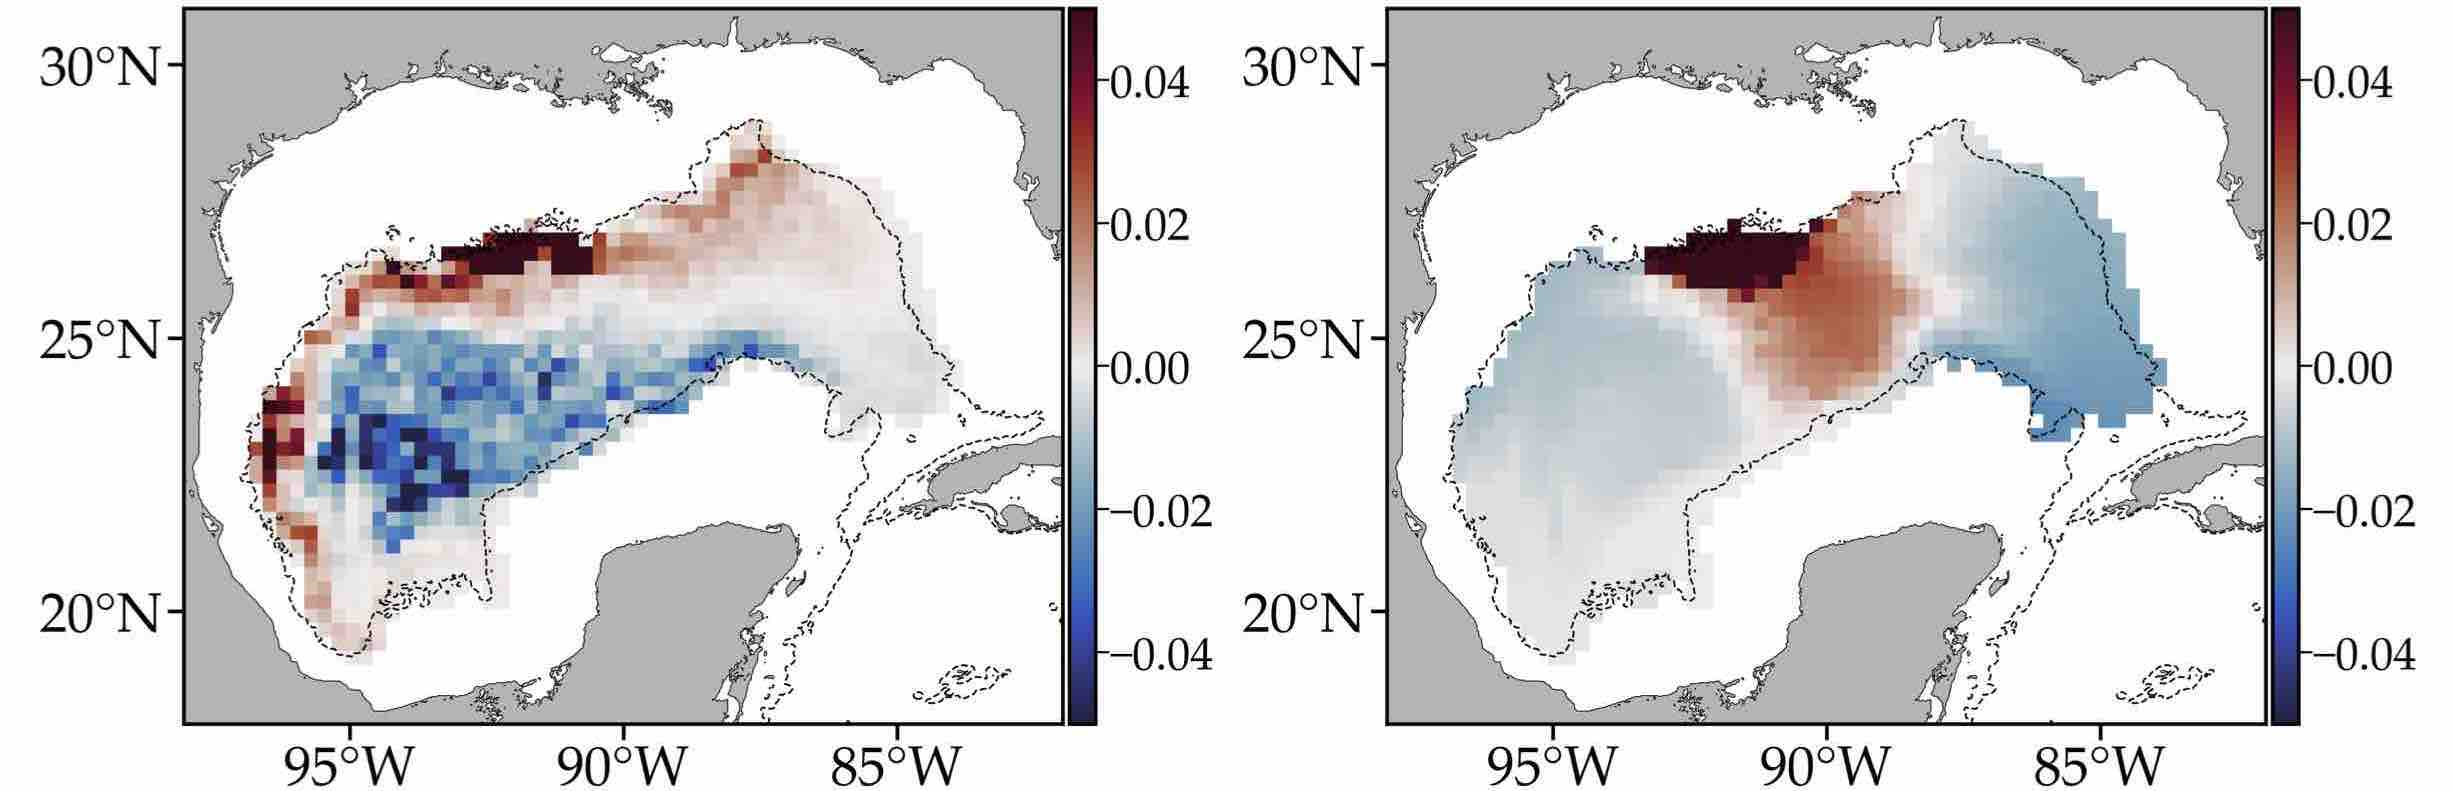
\includegraphics[width=\textwidth]{geogomdeep-fig08b.jpg}
\end{figure}
\begin{figure}
  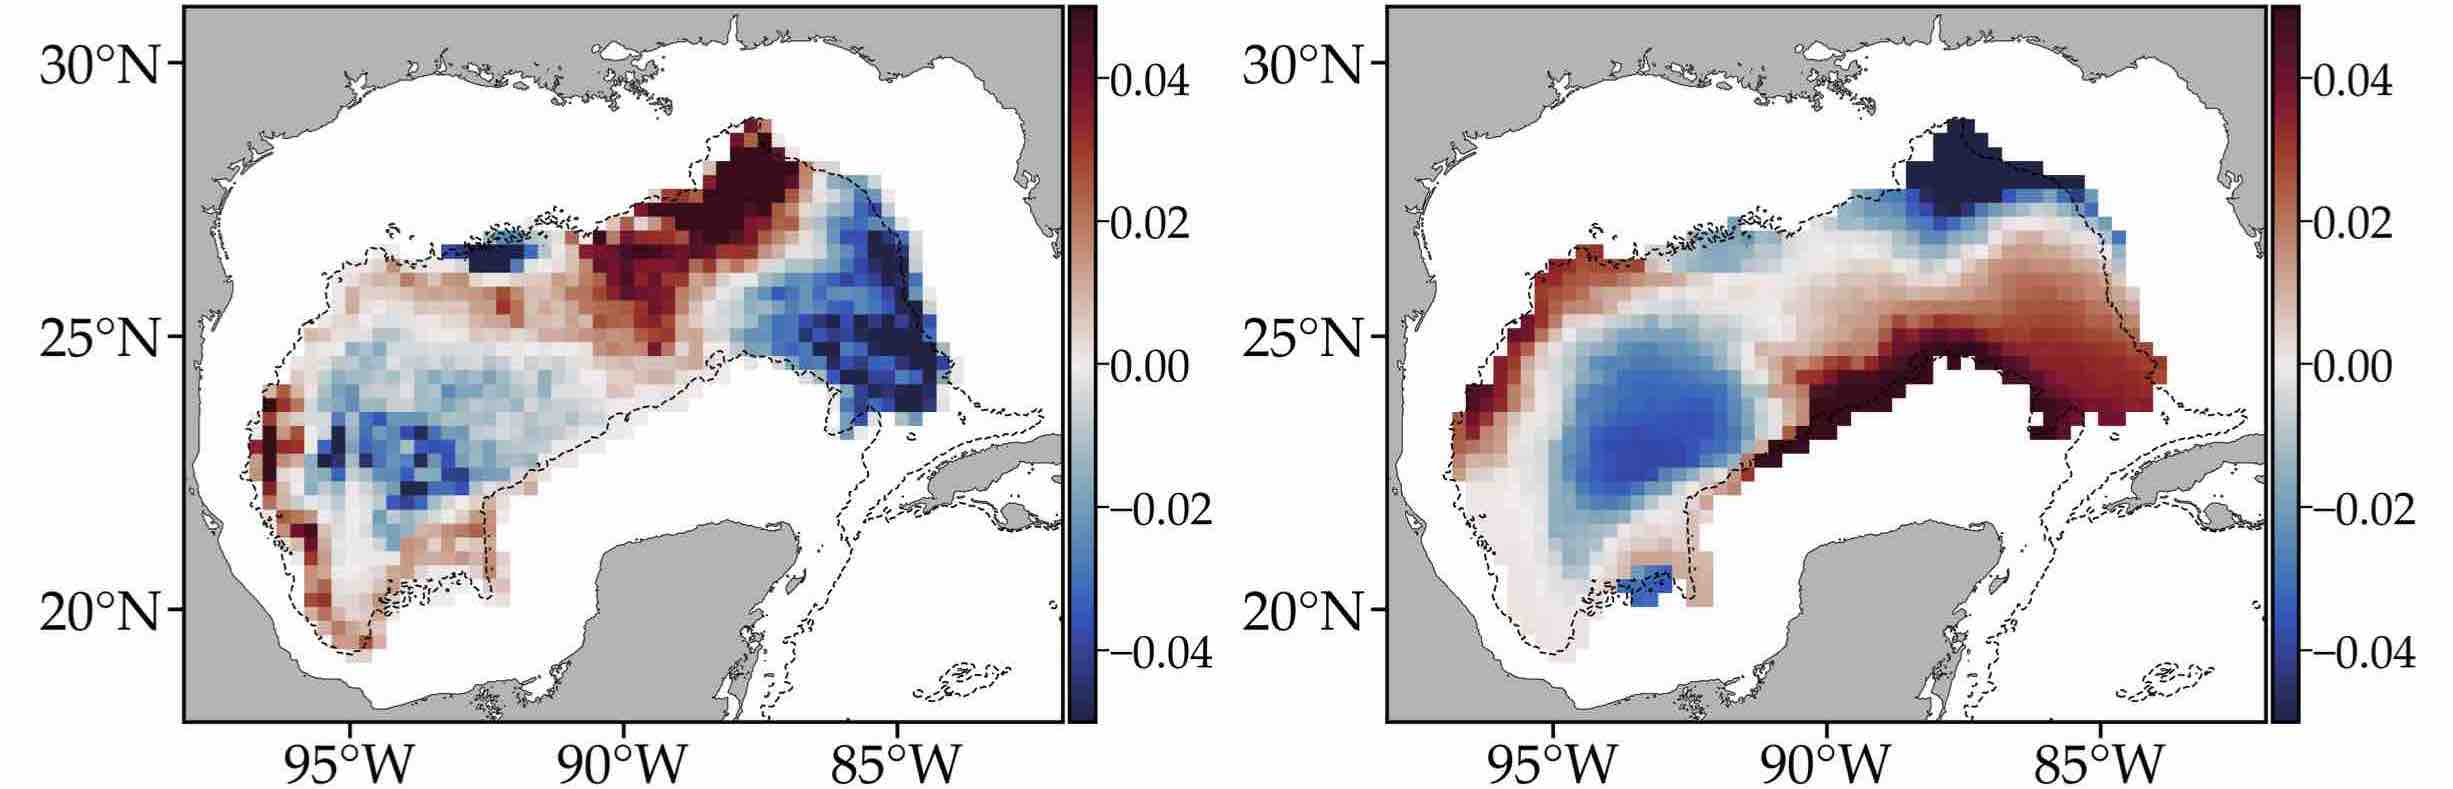
\includegraphics[width=\textwidth]{geogomdeep-fig08c.jpg}
\end{figure}
}
}

\frame{\frametitle{Lagrangian geography of the deep Gulf of Mexico}

Combination of the basins of attraction from the top right eigenvectors (by thresholding).
\begin{figure}
  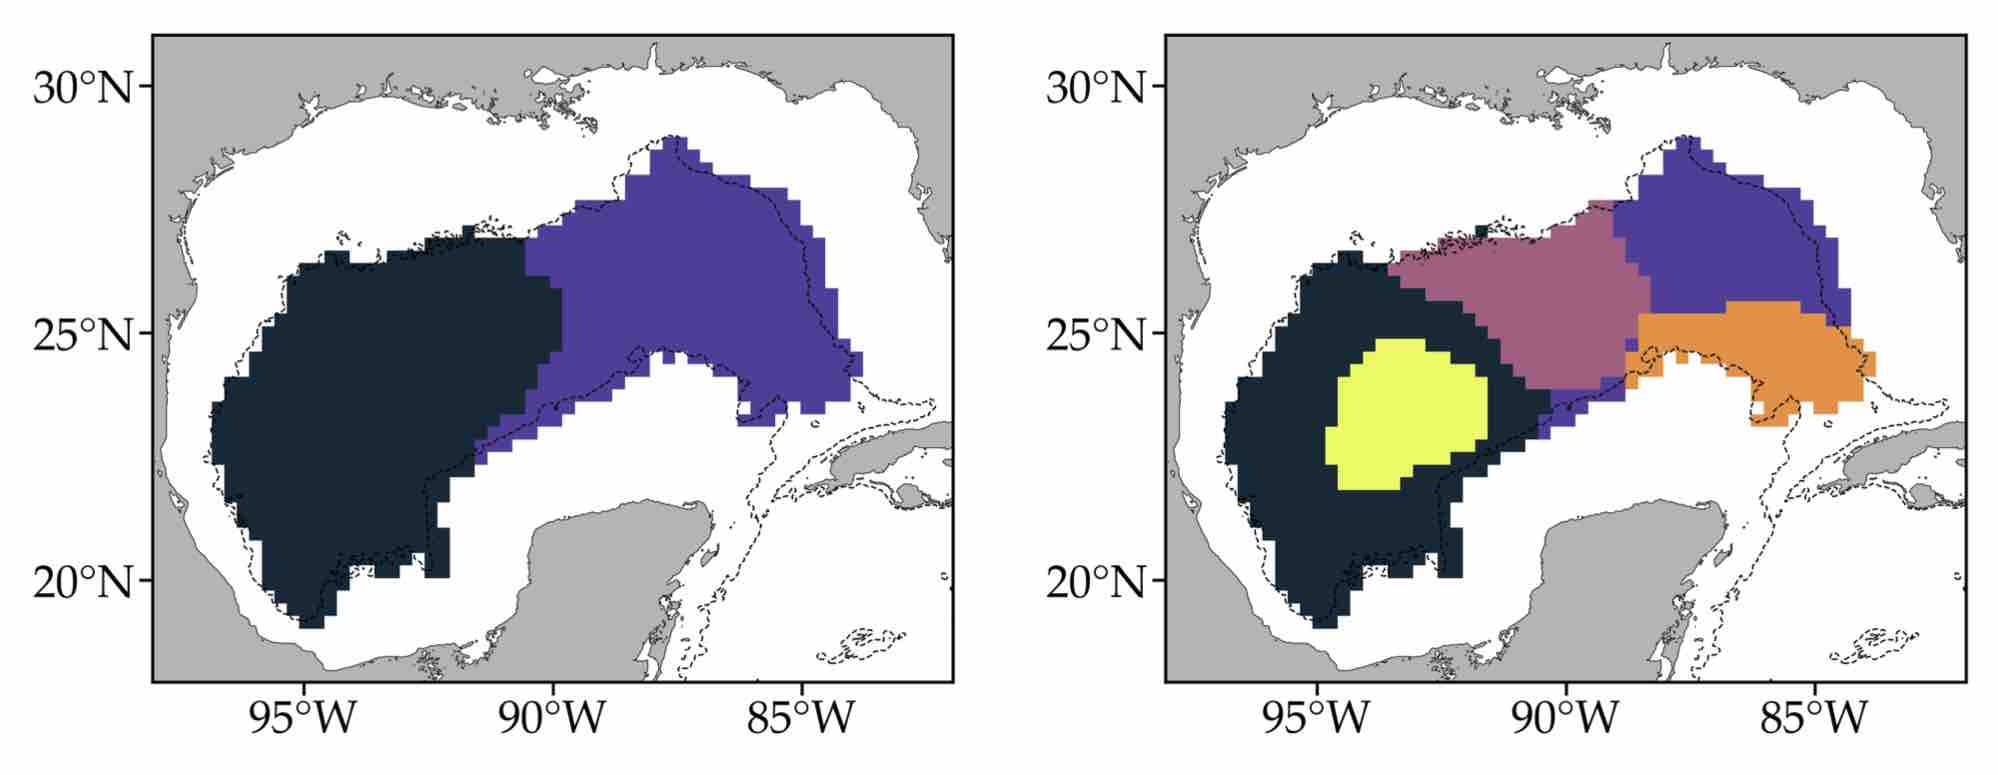
\includegraphics[width=\textwidth]{geogomdeep-fig09.jpg}
\end{figure}

Residence timescale: 7-y left (black) and right (purple), 1-y middle (pink), 0.5-y gyre (yellow) and bottom right (orange)
}

\frame{\frametitle{Residence time}
\begin{figure}
  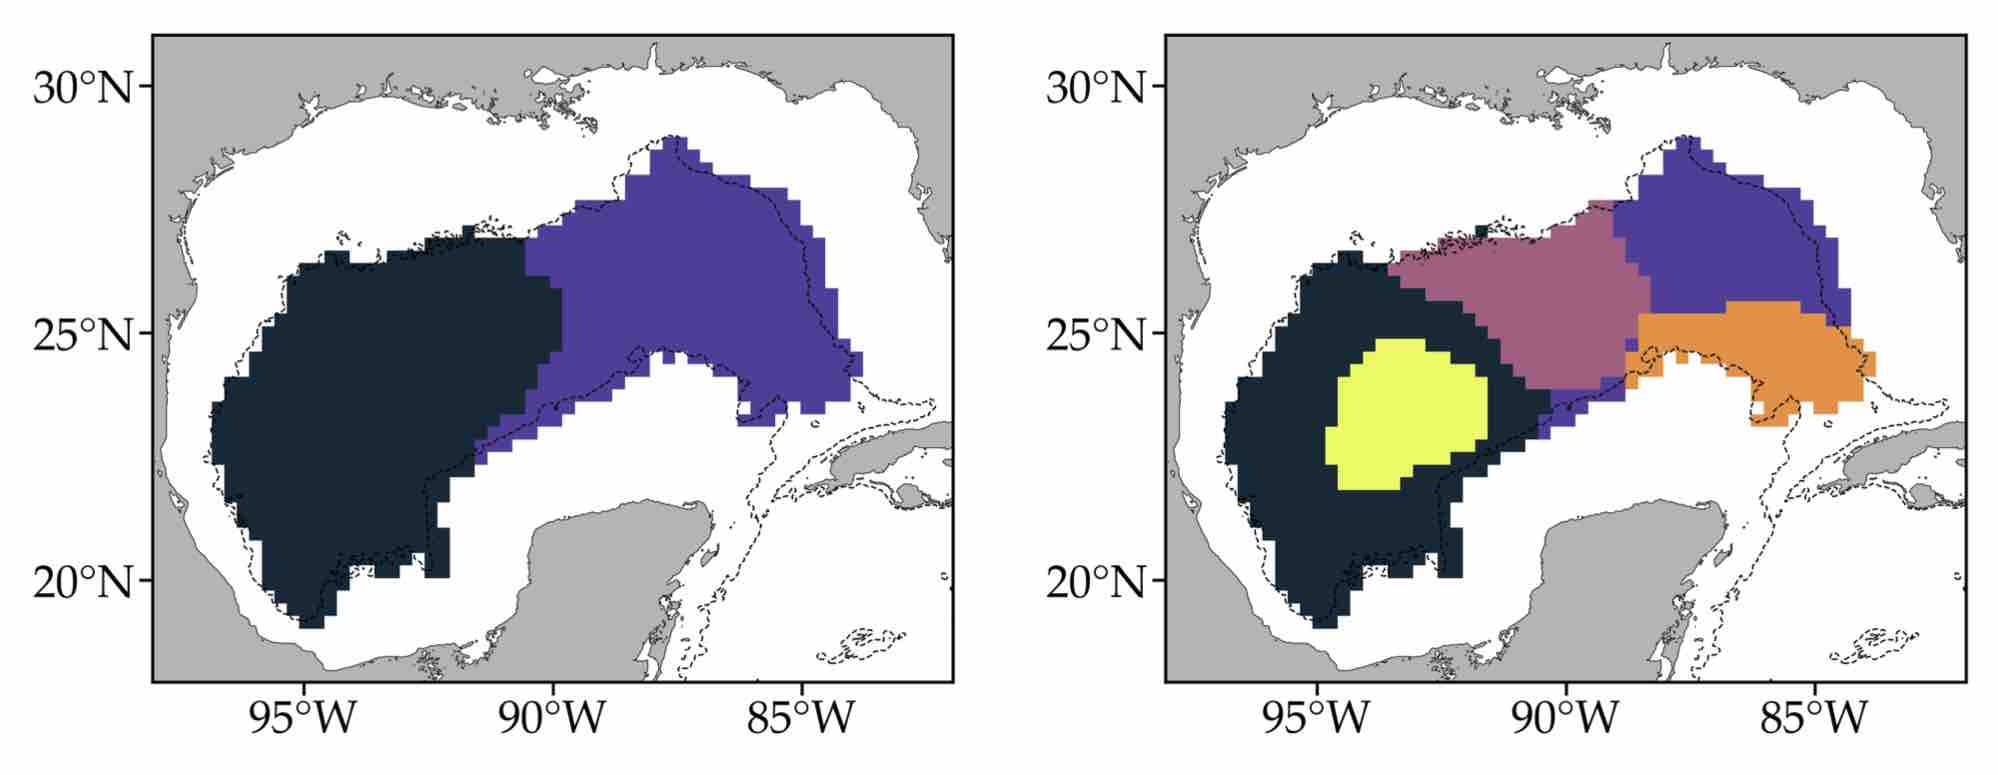
\includegraphics[width=\textwidth]{geogomdeep-fig09.jpg}
\end{figure}
}


\frame{\frametitle{Connectivity matrix (1, 2, 4 weeks)}
\begin{figure}
  \only<1>{
  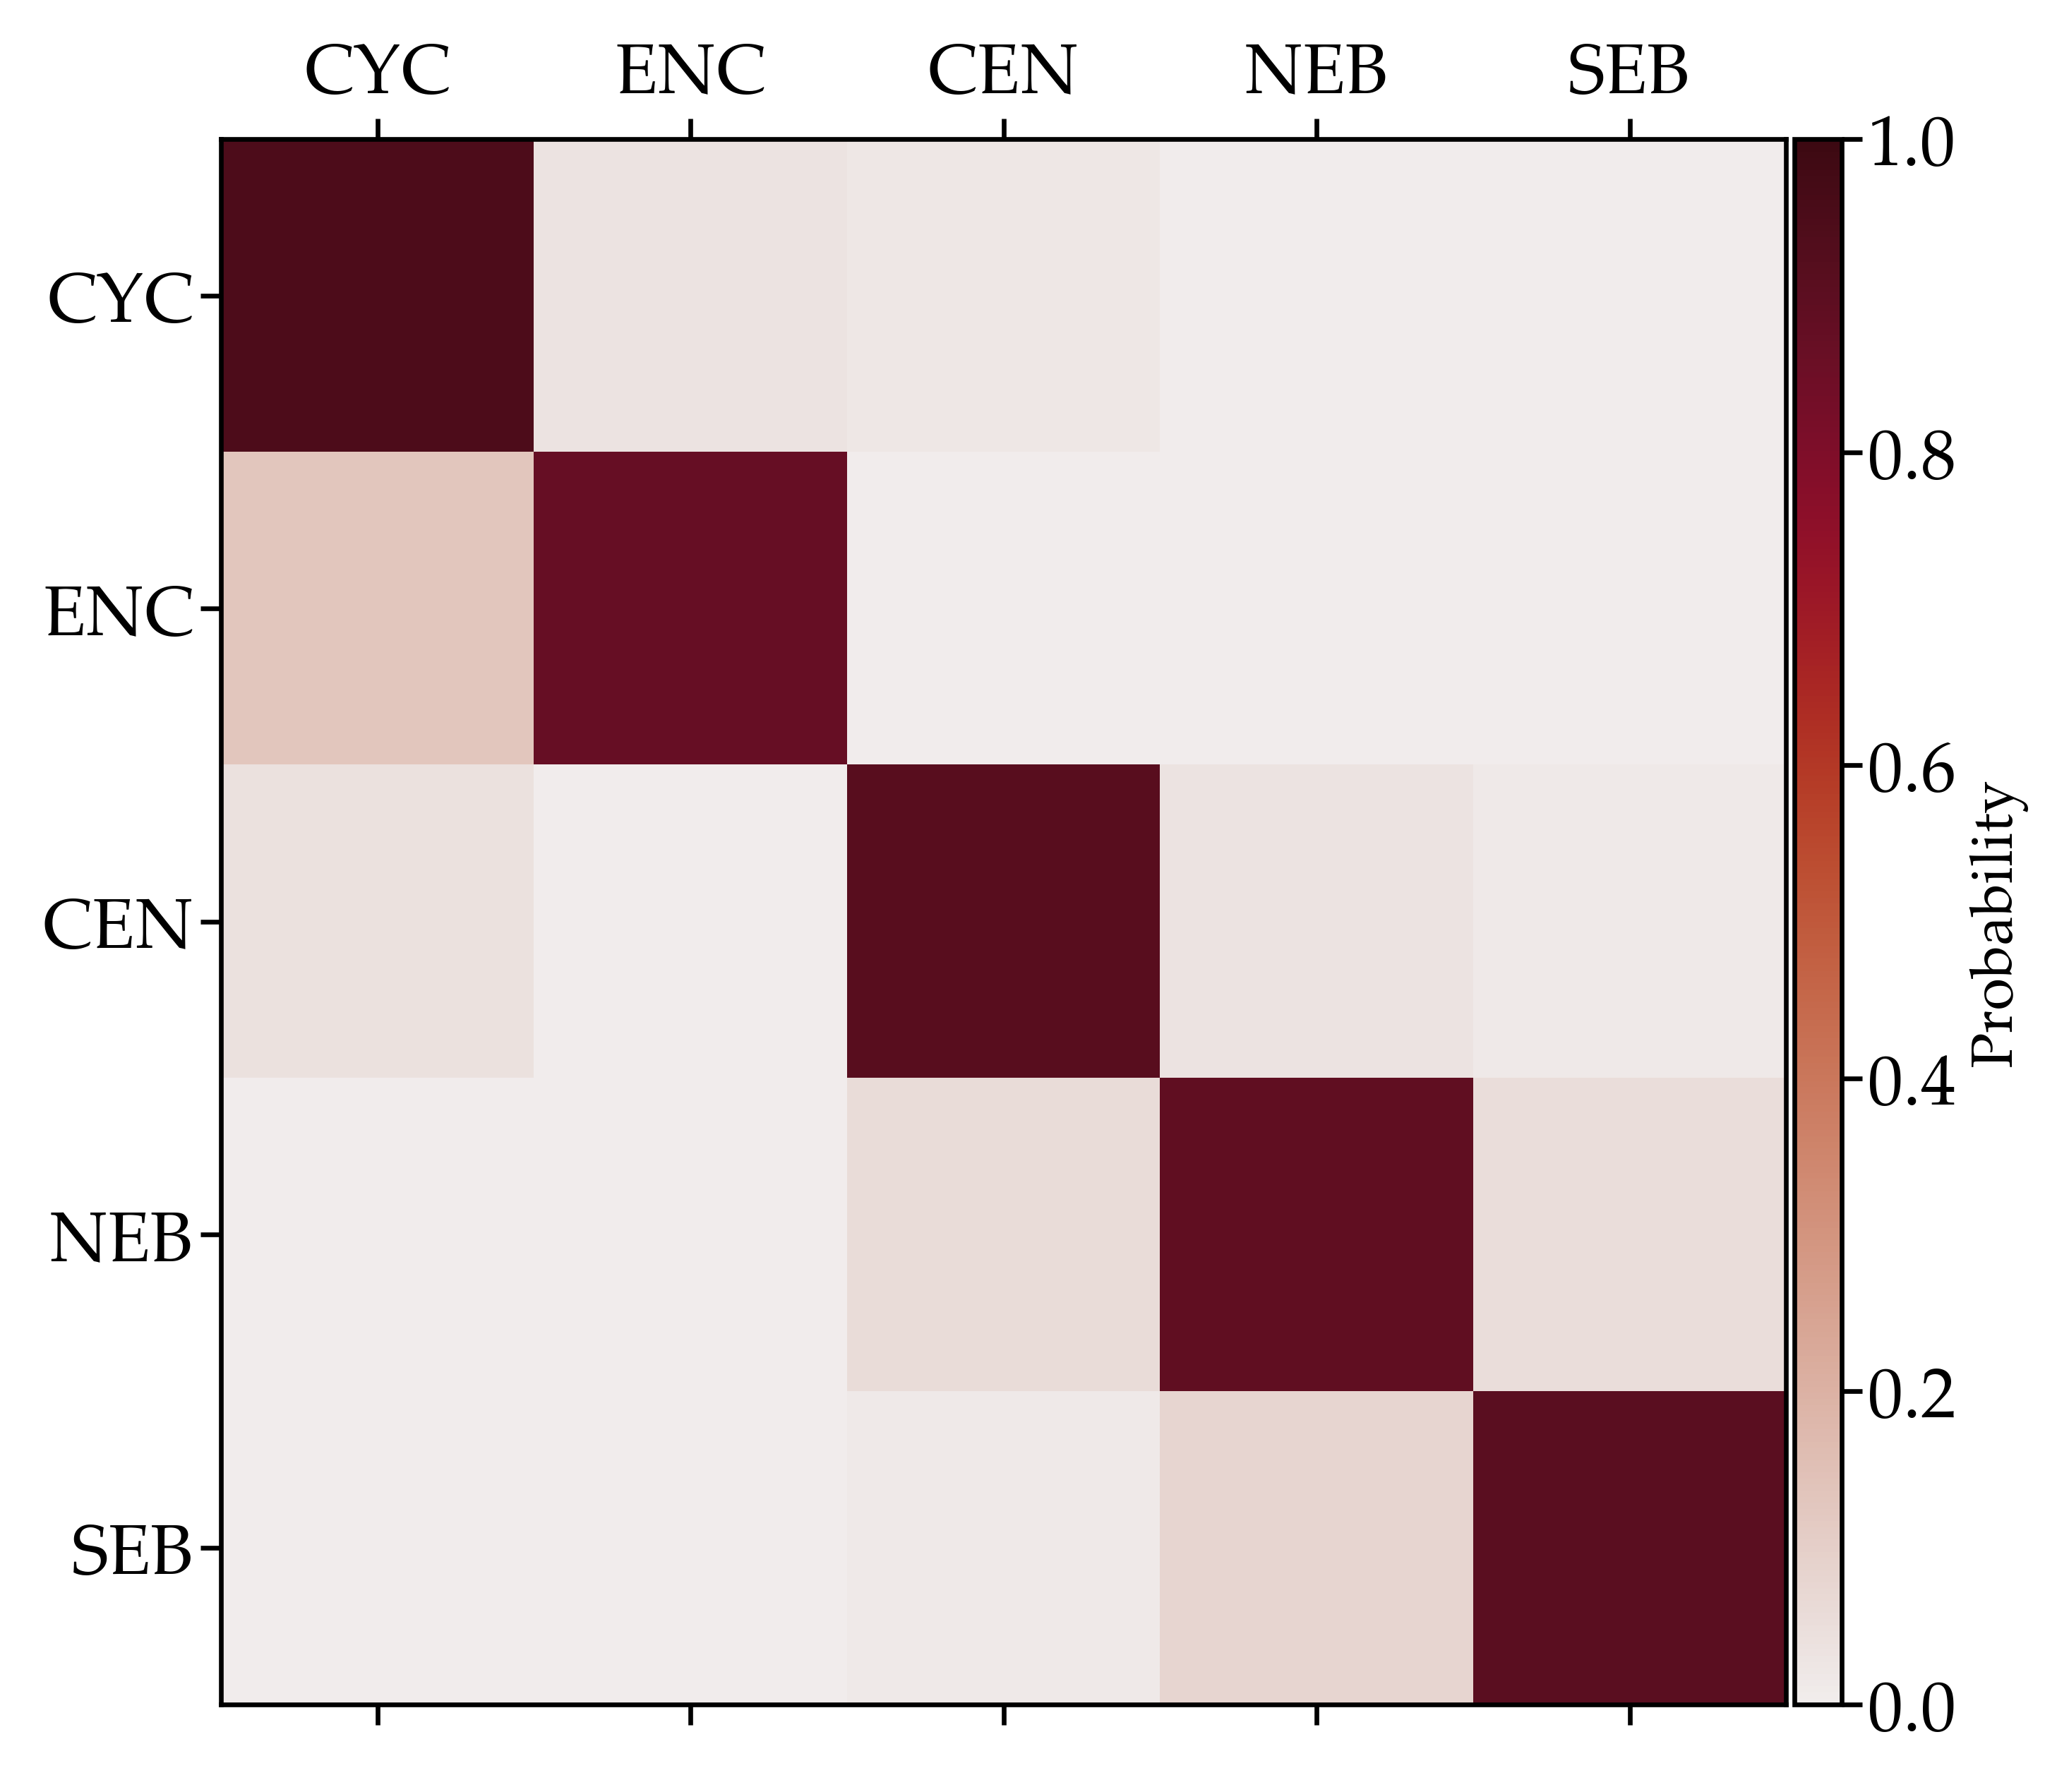
\includegraphics[width=0.9\textwidth]{1wconnection.png}
  }
  \only<2>{
  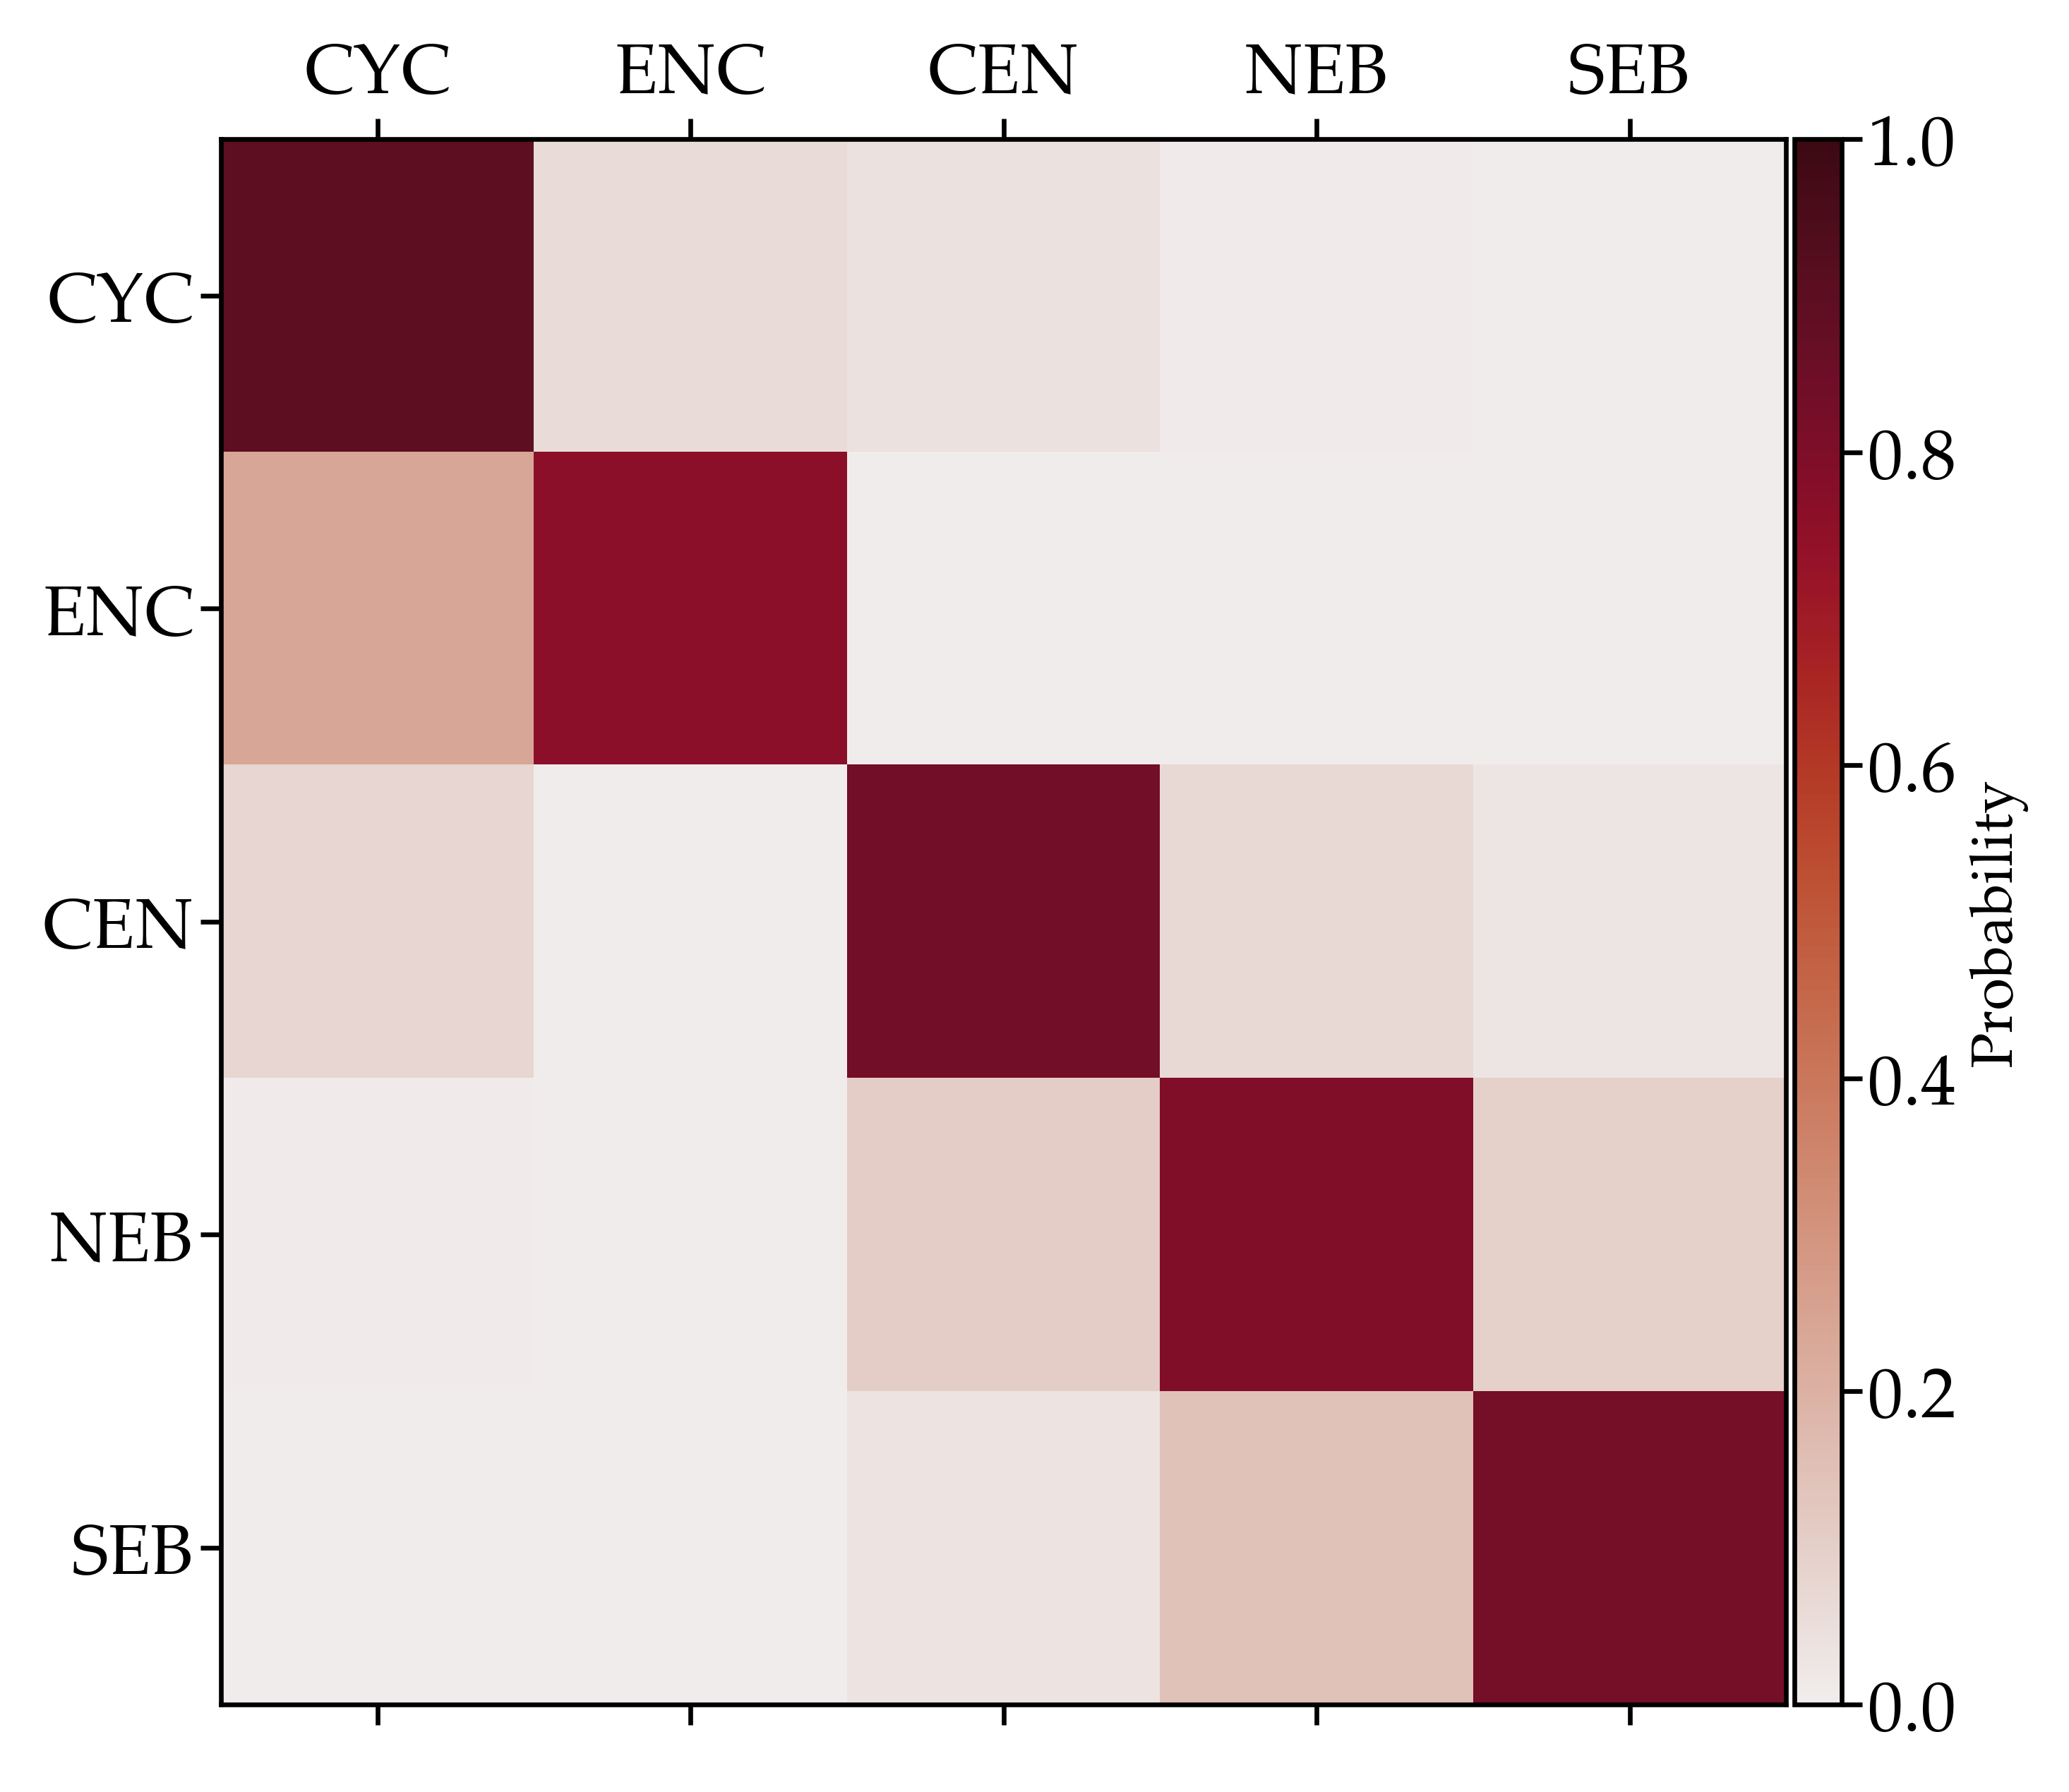
\includegraphics[width=0.9\textwidth]{2wconnection.png}
  }
  \only<3>{
  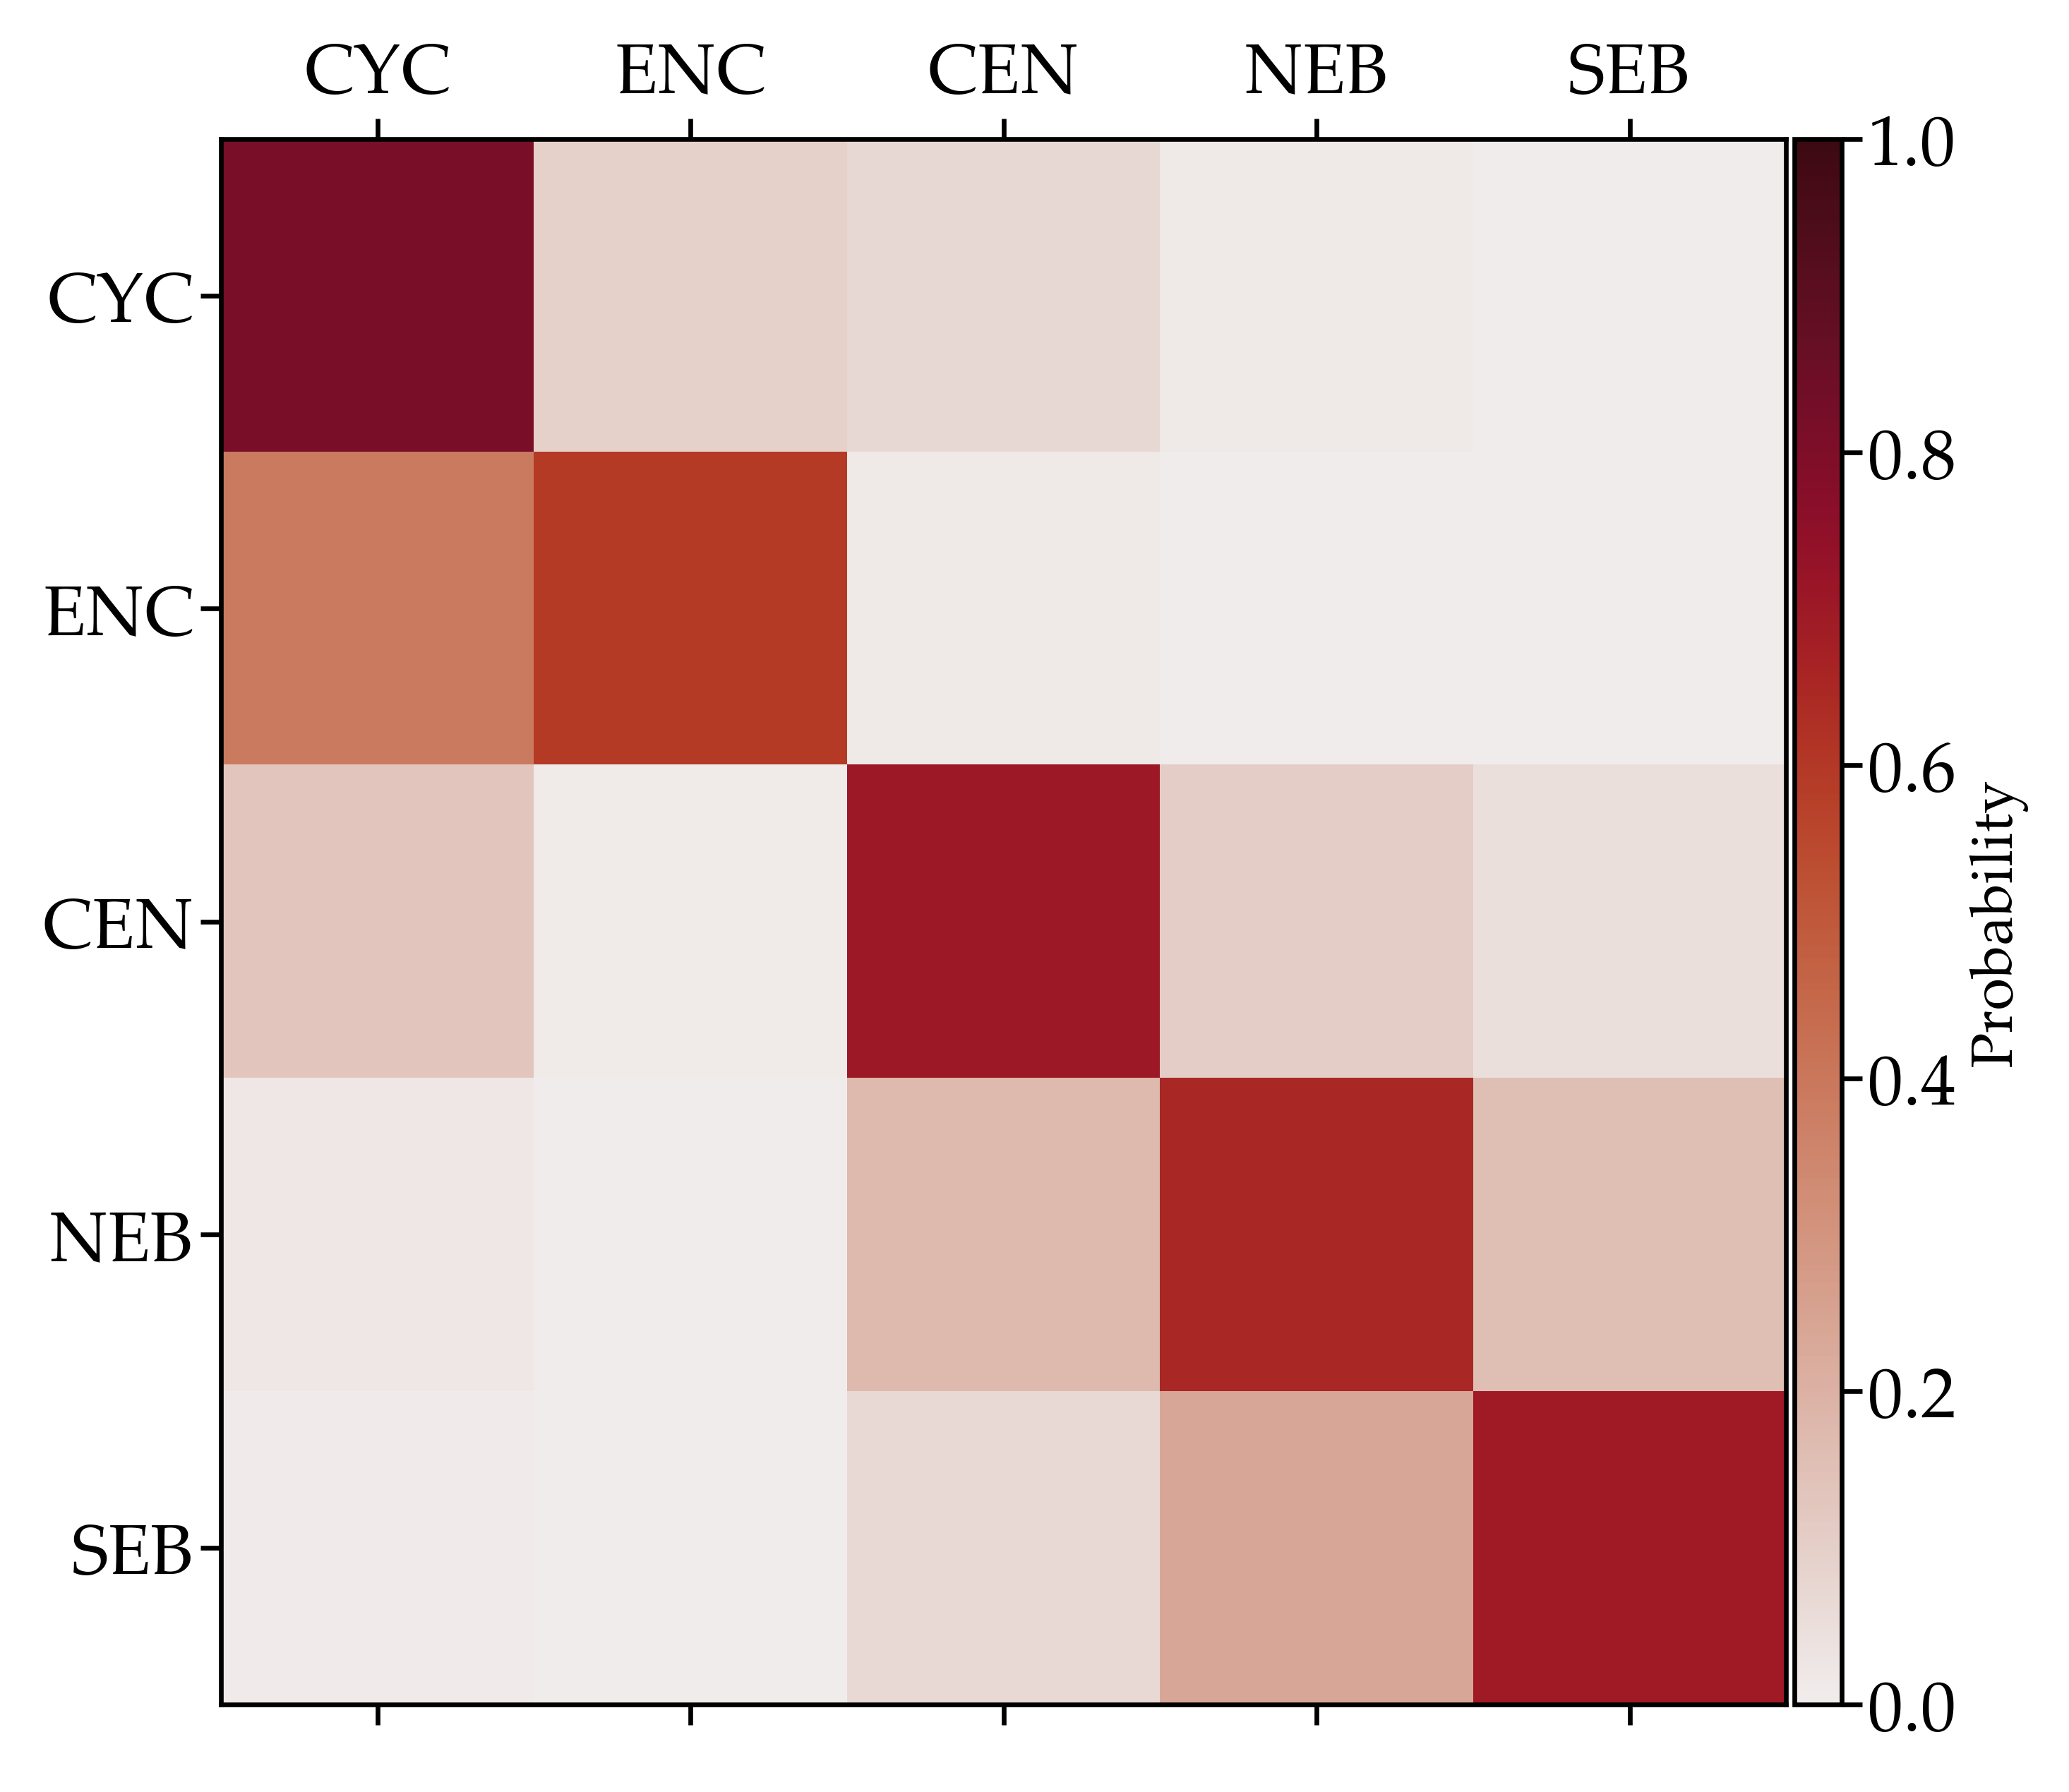
\includegraphics[width=0.9\textwidth]{4wconnection.png}
  }
\end{figure}
}

\frame{\frametitle{Mean expected hitting time}
The time $\tau$ for a trajectory in box $B_i$ to move out of $A$, also known also as the mean time to hit the complement of $A$ \citep{Norris-98}.
\begin{equation} 
  (\Id - P|_A)\tau/T = \mathbf{1},
  \label{eq:tau}
\end{equation} 
\begin{figure}
    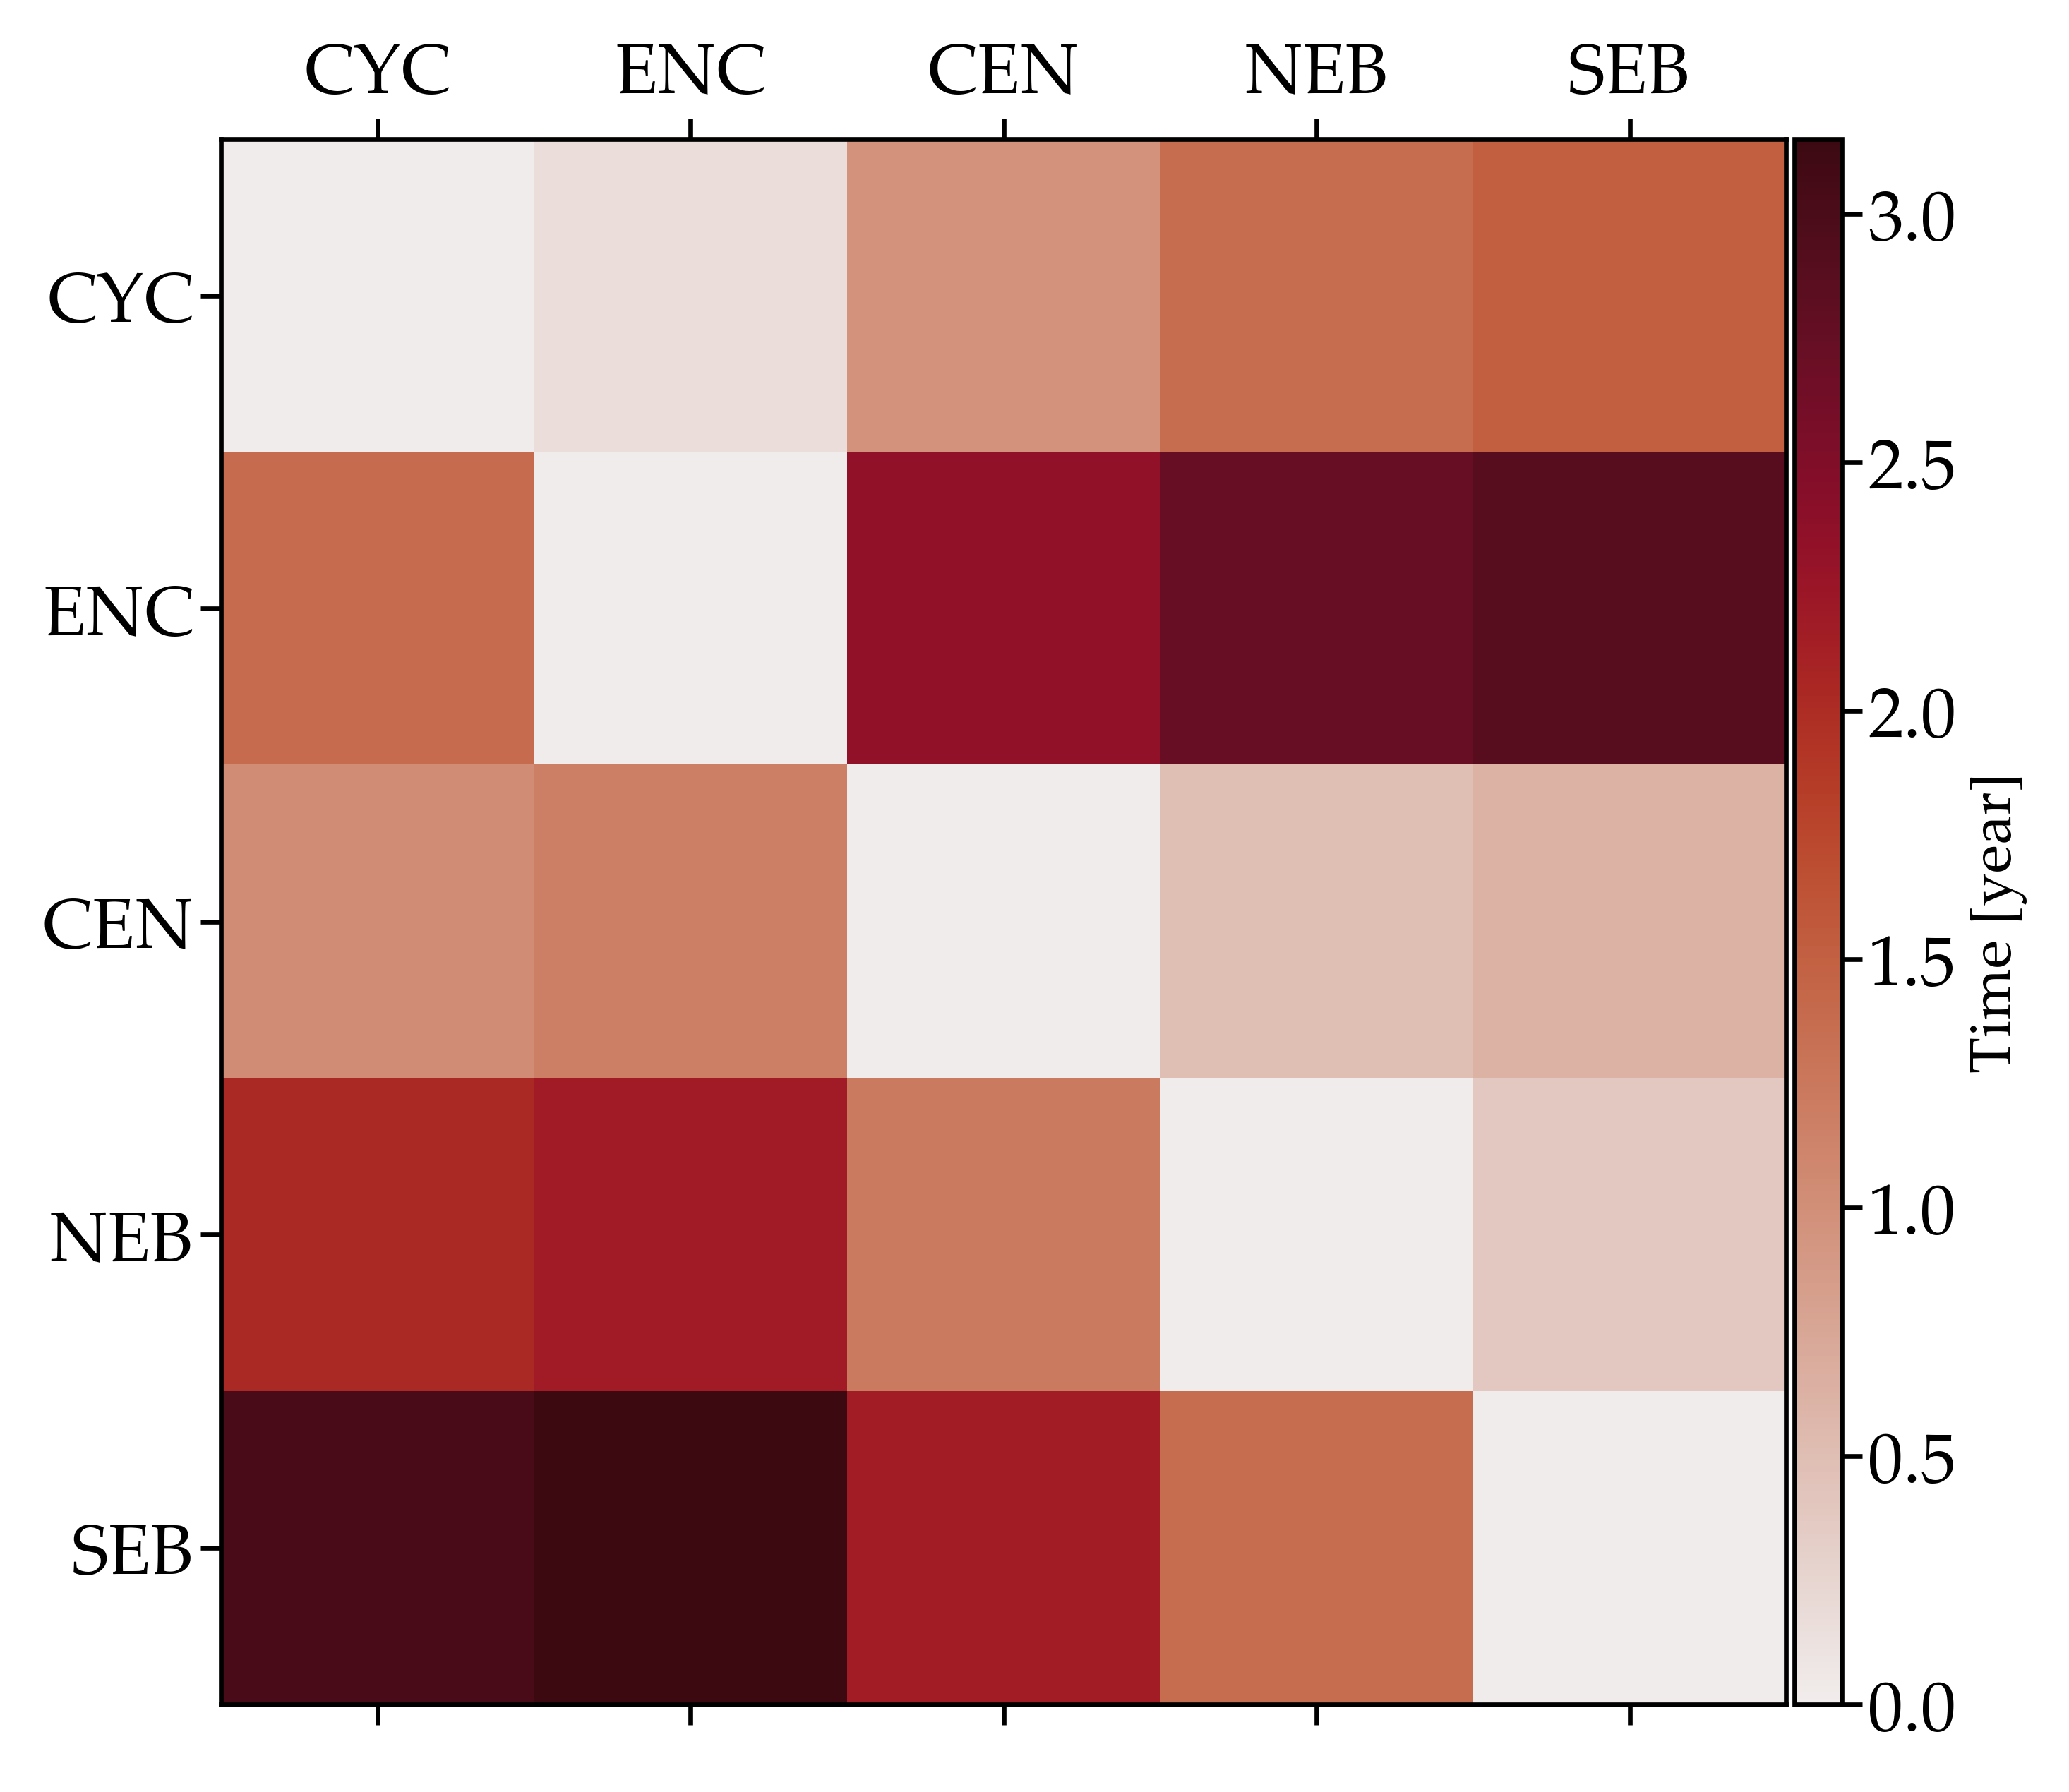
\includegraphics[width=0.7\textwidth]{hitting_time.png}
\end{figure}
}

\frame{\frametitle{Upwelling and Downwelling}
From incompressibility, accumulation can be used to approximate vertical velocity $w$:
\begin{equation}
    h_{t_1} = h_{t_0} \frac{\area_{t_0}}{\area_{t_1}} \quad w \sim \frac{h_{t_1} - h_{t_0}}{dt}. 
\end{equation}

\begin{figure}
  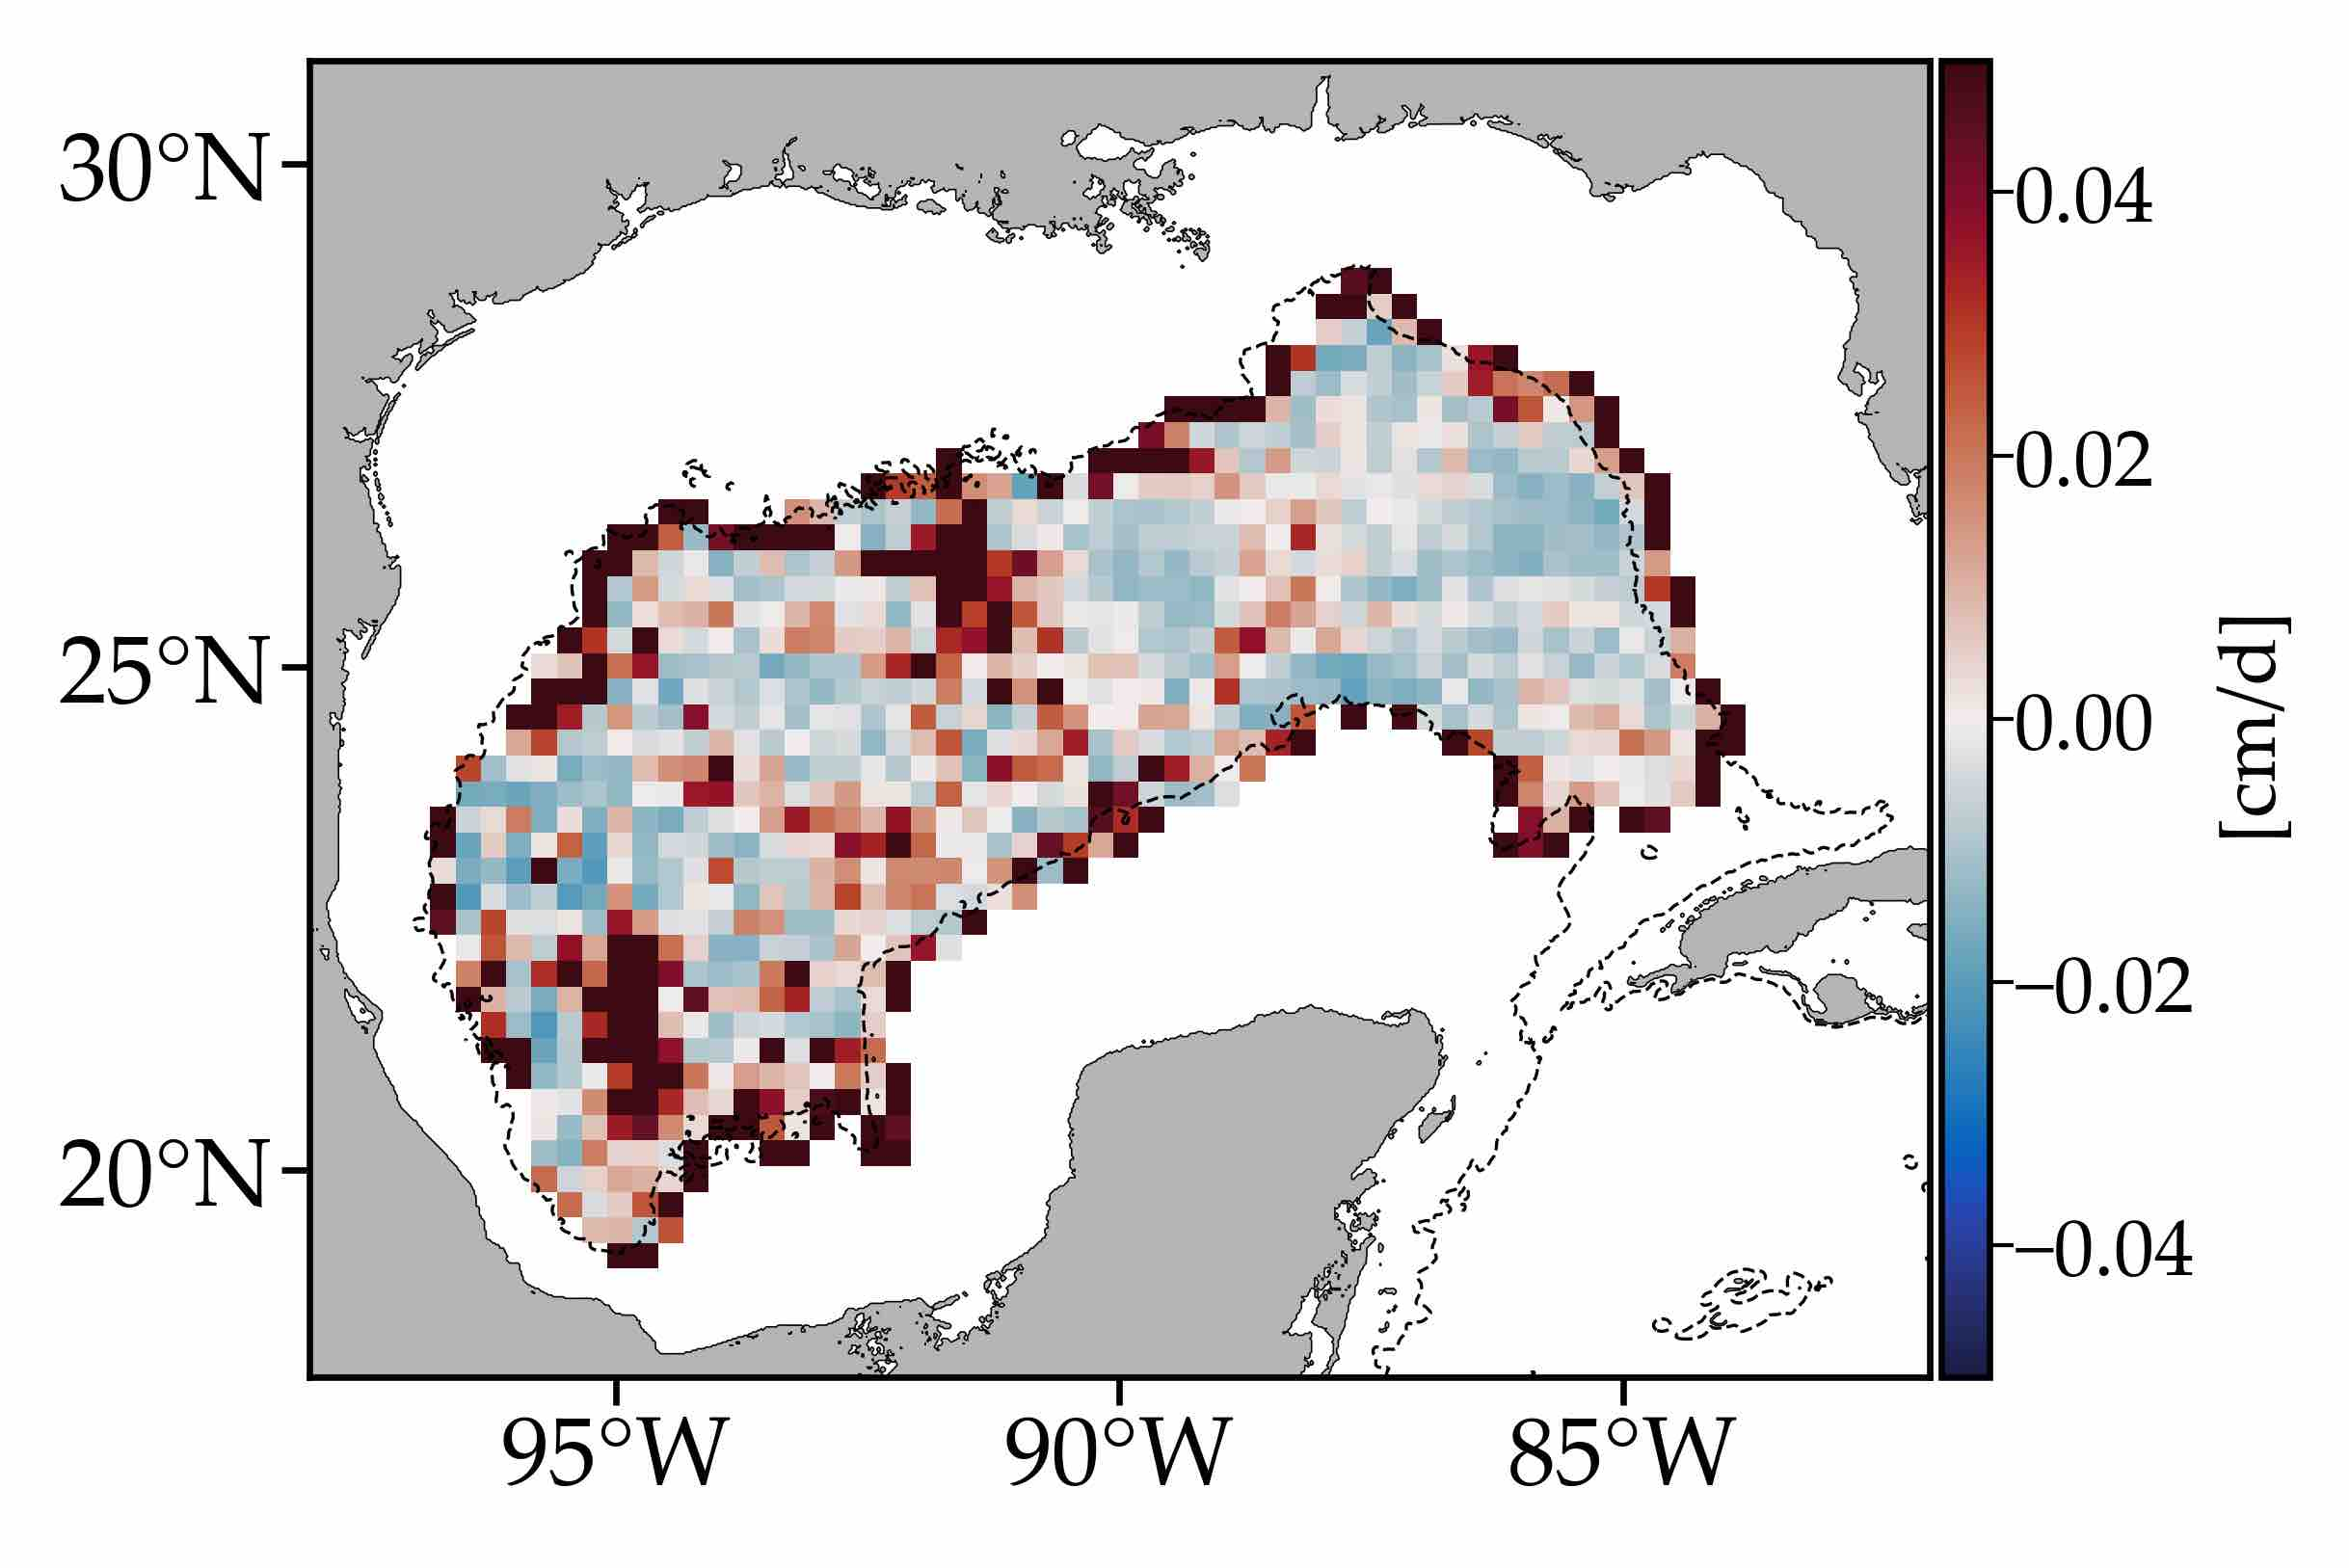
\includegraphics[width=8.5cm]{geogomdeep-fig05.jpg}
\end{figure}

The vertical component is about $\sim 1\%$ of the maximum horizontal velocity ($u_{max} = 0.2739$m/s, $v_{max} = 0.1790$m/s).
}

\frame{\frametitle{Comparison with experimental data \citep{ledwell2016dispersion}}

\only<1>{
Tracer evolution from the infamous Deepwater Horizon oil spill.
\begin{figure}
  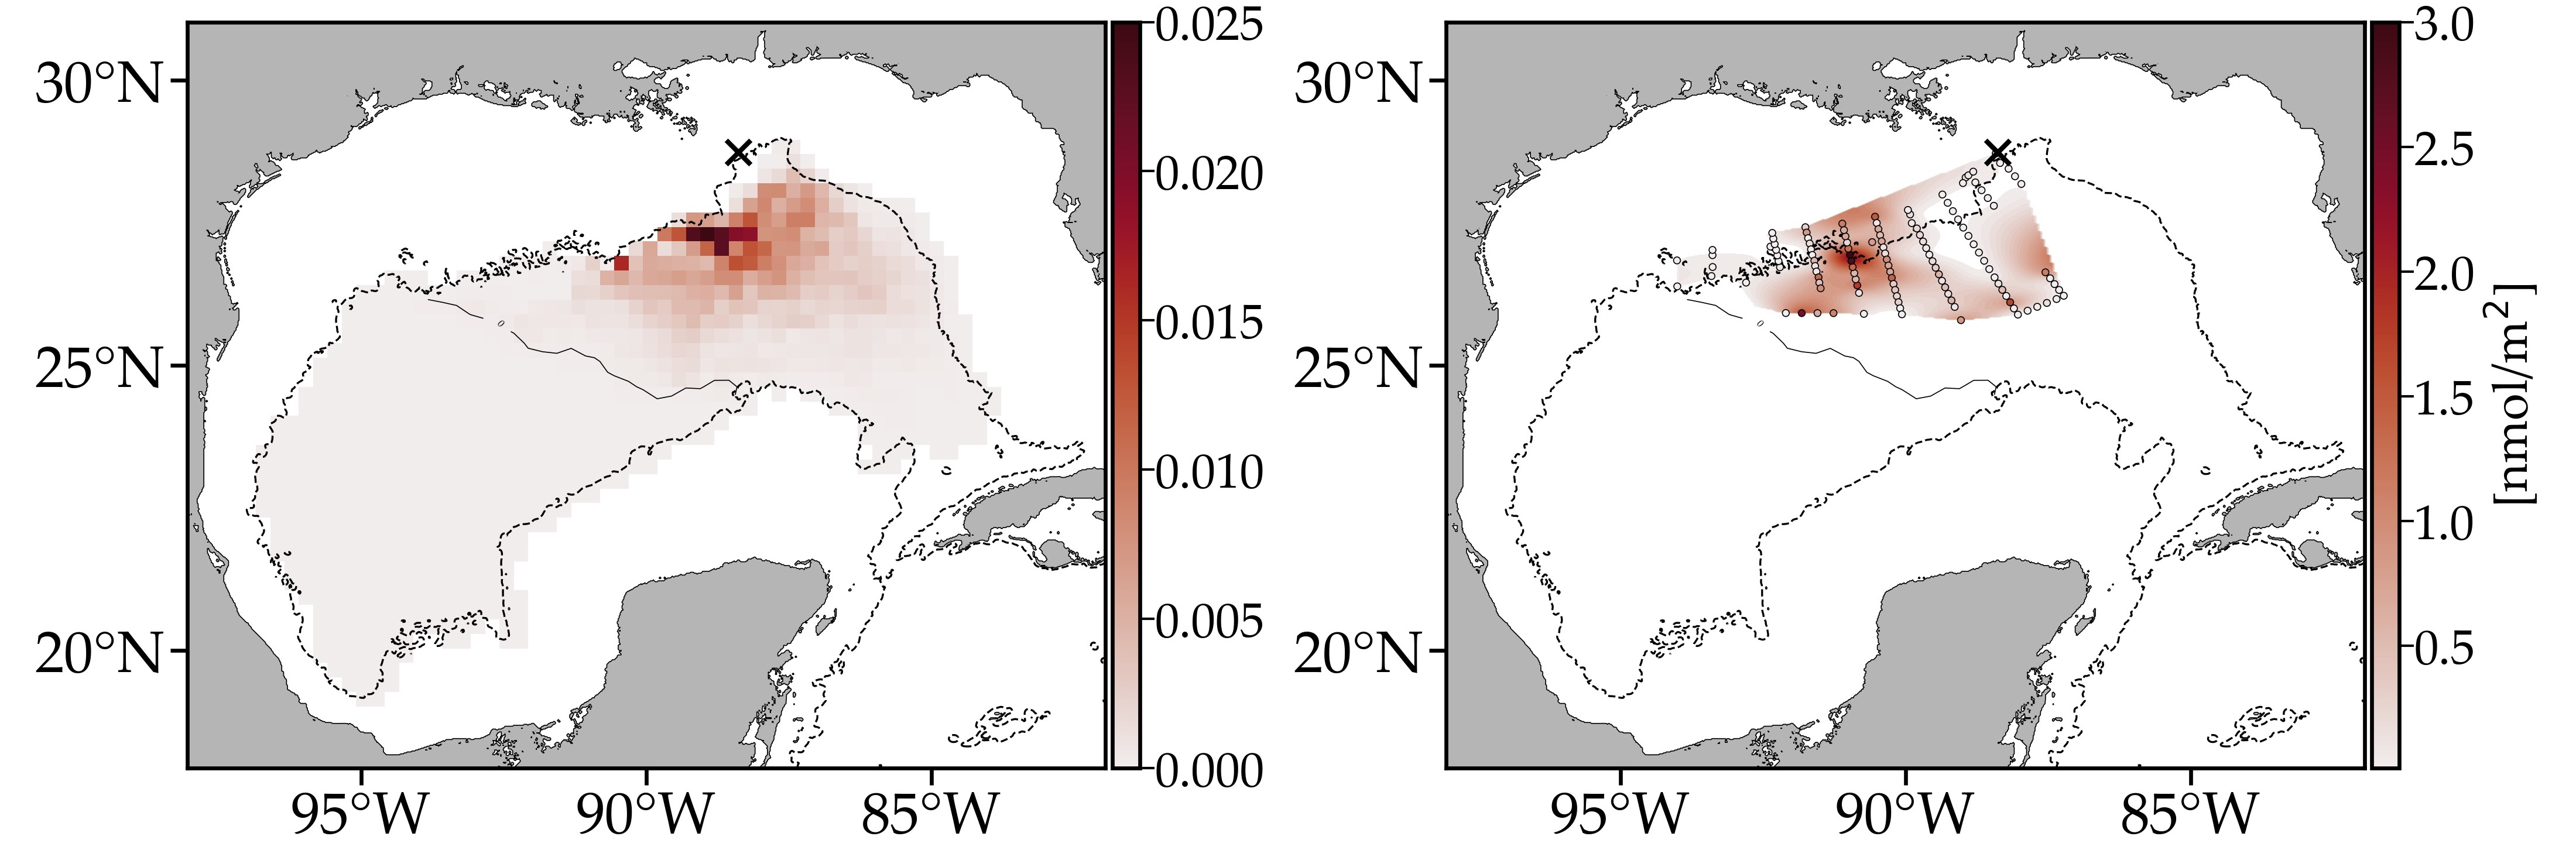
\includegraphics[width=\textwidth]{geogomdeep-fig11.jpg}
  \caption{Evolution after 4 months}
\end{figure}
}

\only<2>{
\begin{figure}
  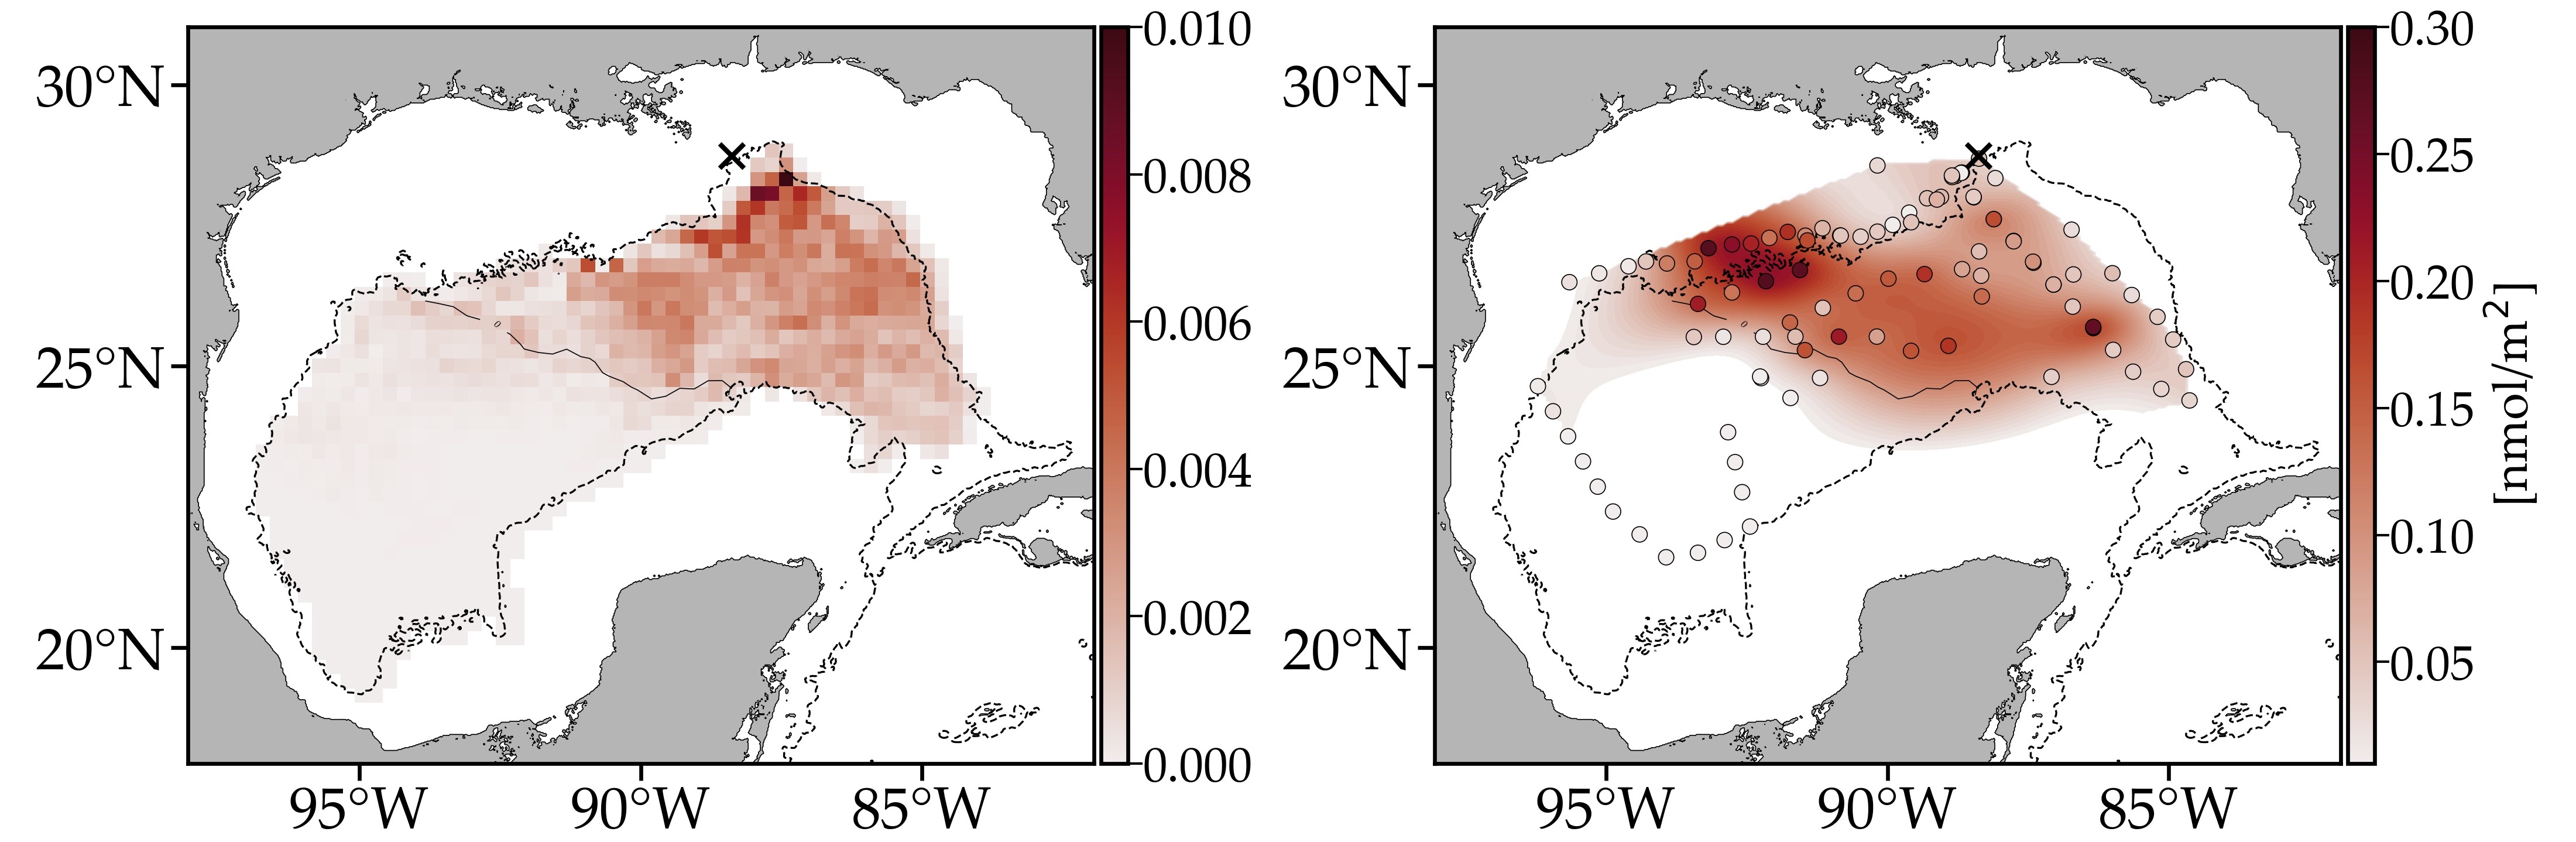
\includegraphics[width=\textwidth]{geogomdeep-fig11b.jpg}
  \caption{Evolution after 12 months}
\end{figure}
}
}

\frame{\frametitle{Argo floats}
 
\only<1>{

Talk about the entrance ?! No floats exit ?
\begin{figure}
  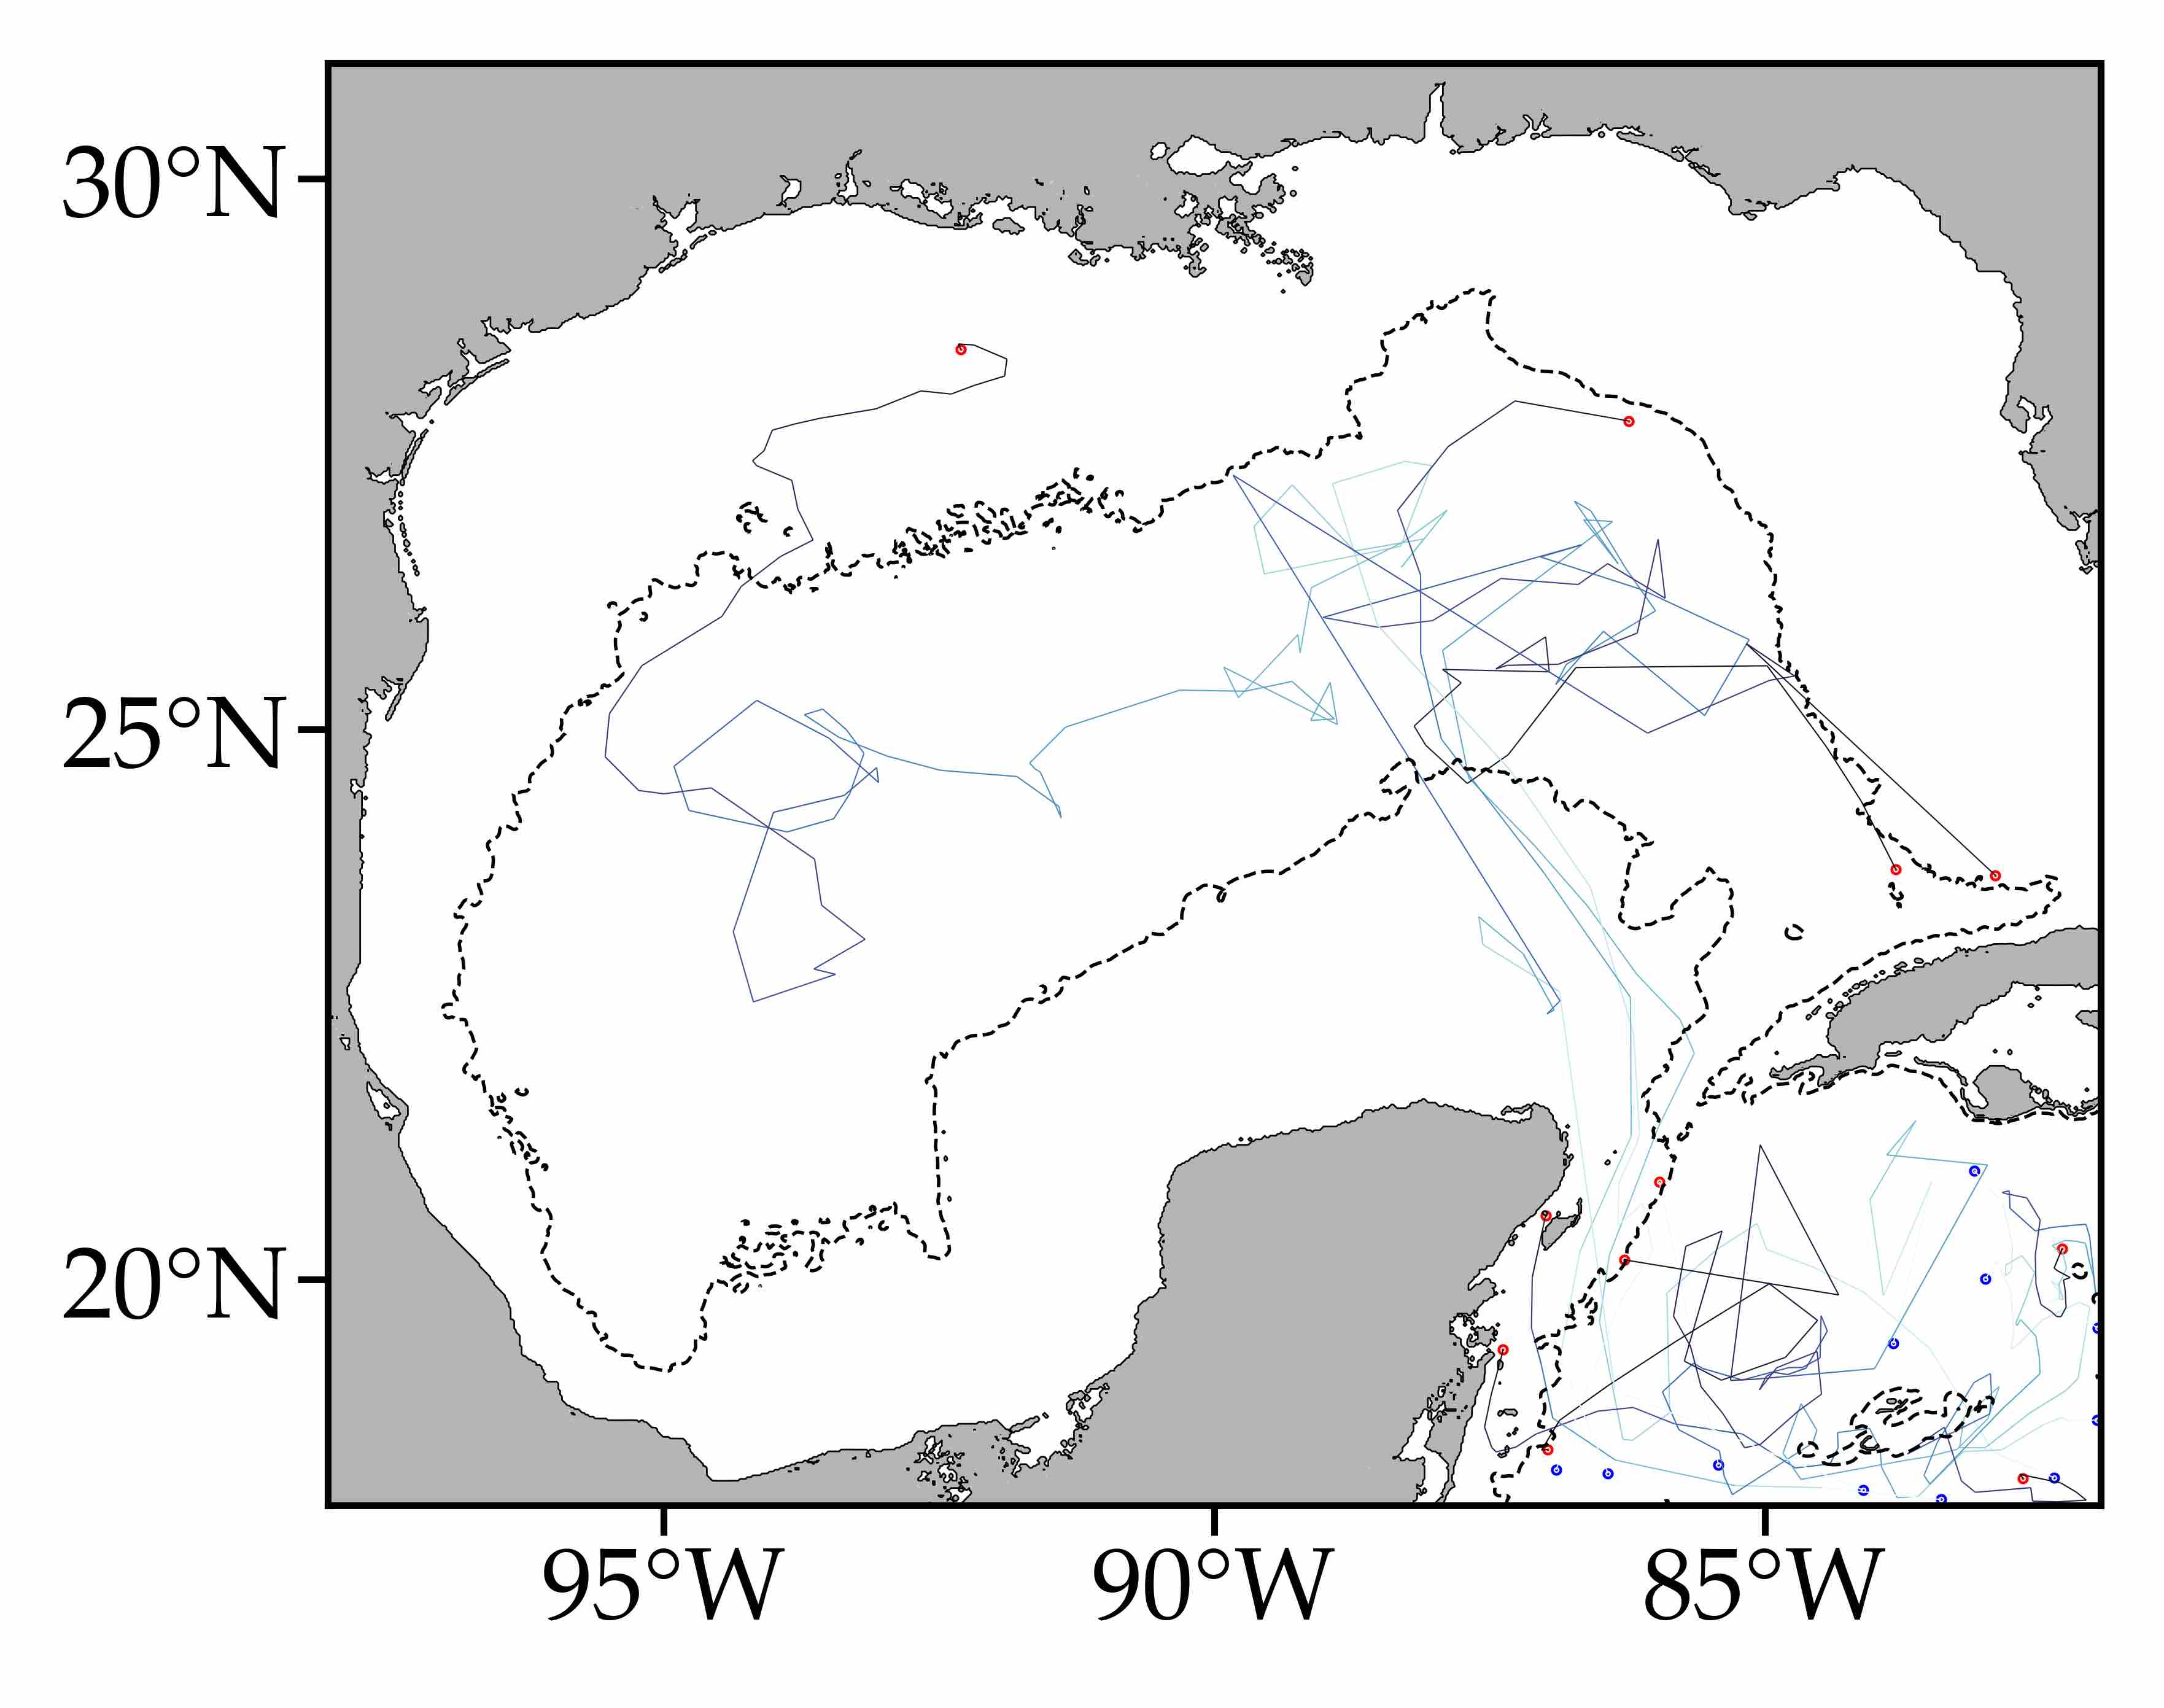
\includegraphics[width=10cm]{geogomdeep-fig13.jpg}
\end{figure}
}

\only<2>{
\begin{figure}
  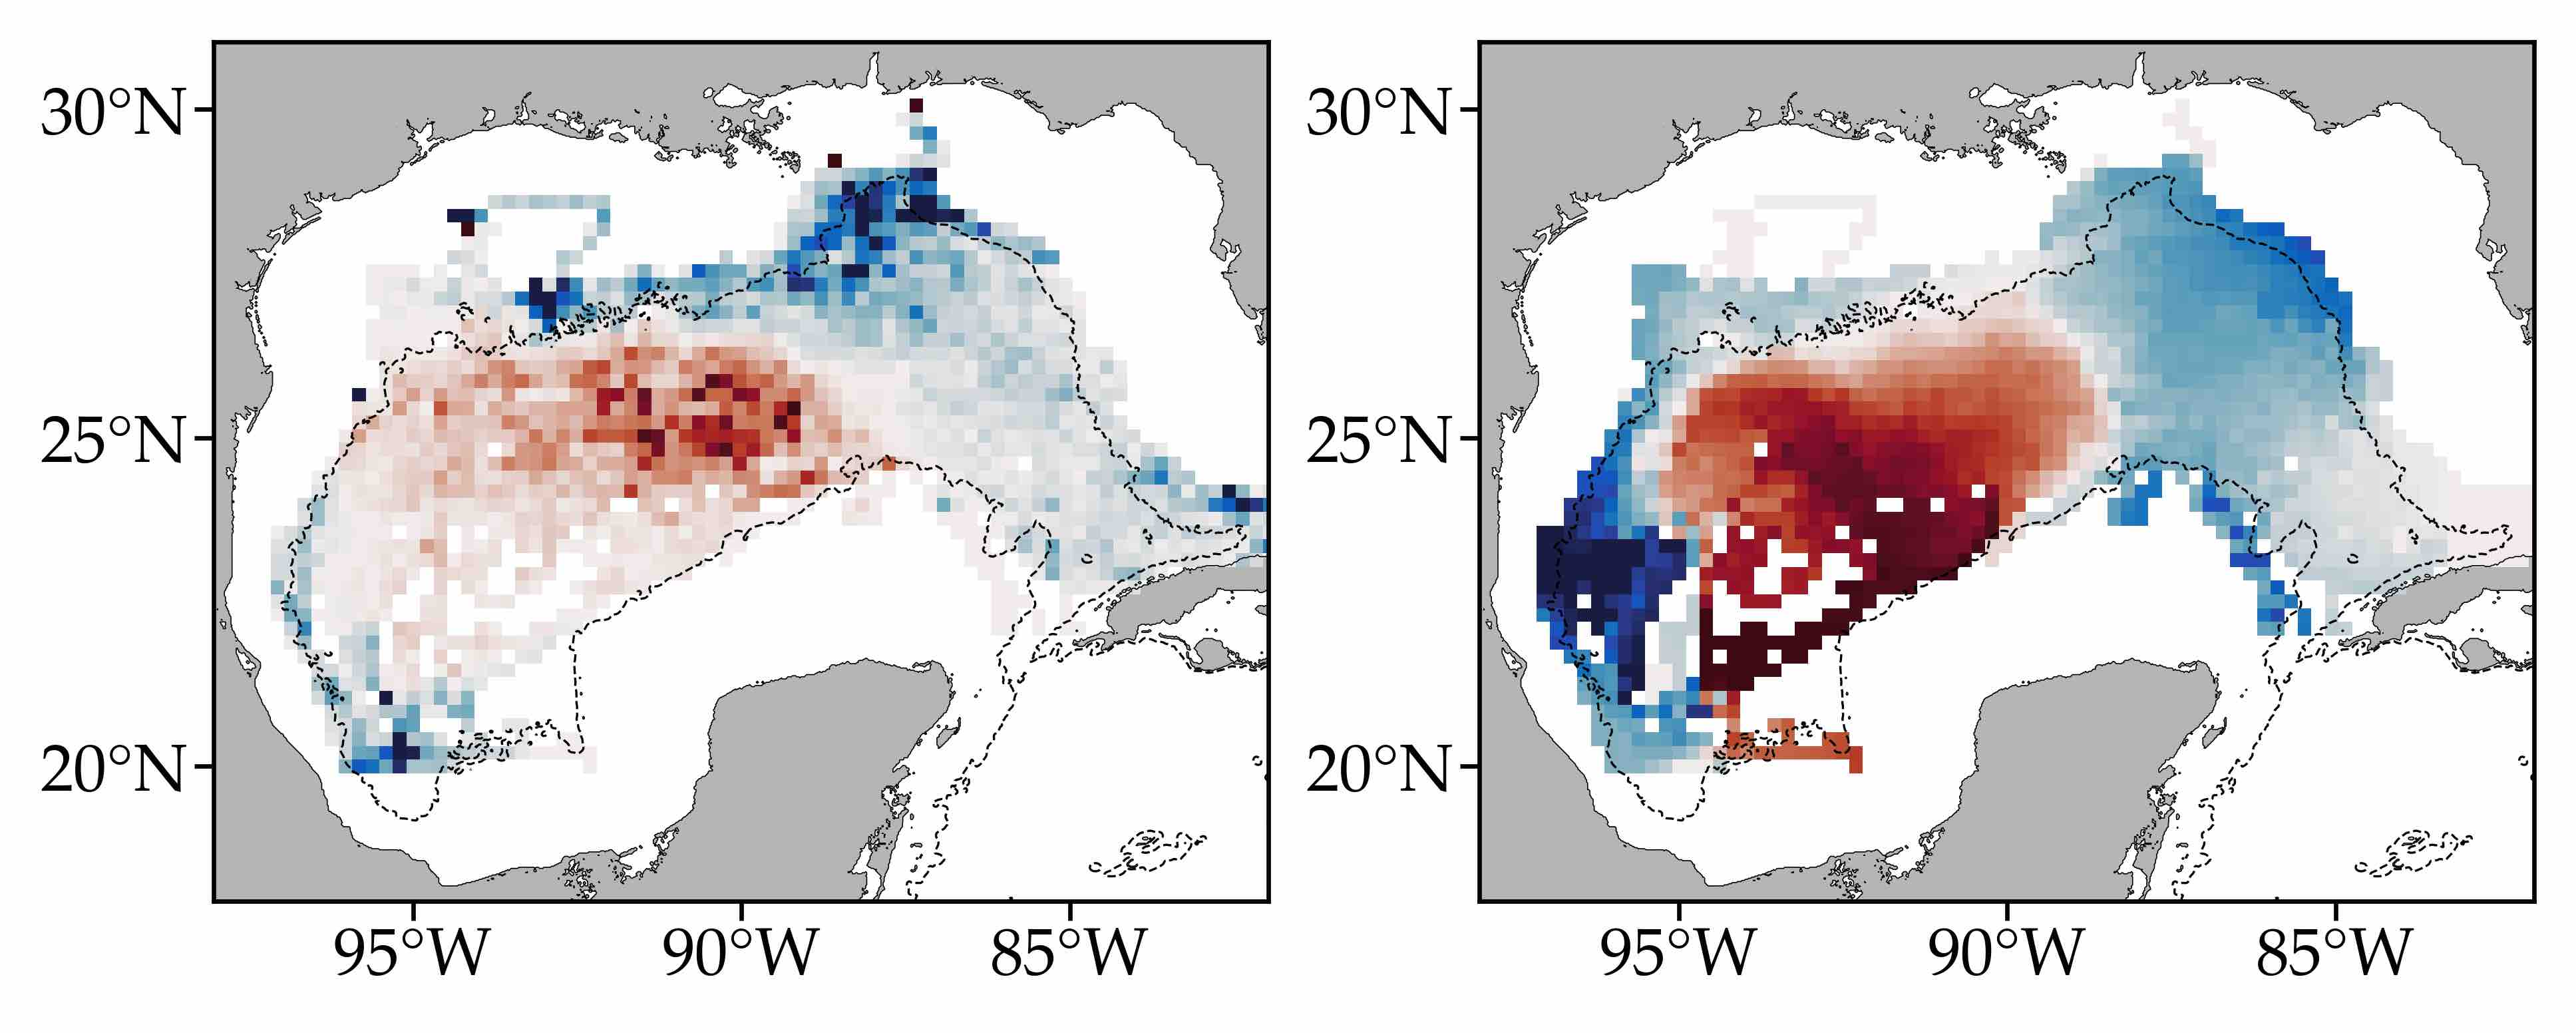
\includegraphics[width=\textwidth]{geogomdeep-fig12.jpg}
  \caption{Argo floats}
\end{figure}
}


}



\section{Conclusion}
\frame{\frametitle{Thank you!}

Also a special thanks to Julio Paula Pérez Brunius

Paper will be submit this week (we are hoping) !

Future plans:
\begin{itemize}
	\item Evaluation of global circulation from surface drifters and deep water floats
\end{itemize}

Any questions?
}

\frame[allowframebreaks]{\frametitle{References}

% remove References title
\begingroup
\renewcommand{\section}[2]{}%
% add cited papers
\printbibliography[heading=none]
\endgroup
}

\end{document}